%
% Tallinn University of Technology - bachelor, master thesis Éstonian template for LaTeX
%
%
% Public veresion 1.3
% 2023 translated main parts to Estonian (by Ago Luberg)
%
% Public version 1.2
% 2022 Updated by Karl Janson to match the new formatting guidelines
%
% Public Version 1.1
% 2019 Adjusted by Frank Korving for his Bachelor Thesis, with contributions from Sander Arnus
%
% Public version 1.0
% 2010 - 2013 Thijs Nugteren and Joos Buijs for Master Thesis
%
% THIS IS THE MAIN FILE (i.e. compile this file, compiling the others directly won't work)
%

\documentclass[12pt]{report} % Default font size is 12pt, default paper size is a4

% all the other includes etc. are done in the thesis.sty file.
\usepackage{thesis} % thesis formatting

%%%%%%%%%%%%%%%%%%%%%%%%%%%%%%%%%%%%%%%%%%%%%%%%%%%%%%%%%%%%%
% NOTE:                                                     %
%%%%%%%%%%%%%%%%%%%%%%%%%%%%%%%%%%%%%%%%%%%%%%%%%%%%%%%%%%%%%
% * Content chapter files are located in "chapters" folder, %
%   included using the "chapters_main.tex" file             %
%                                                           %
% * Appendices are located in "appendices" folder,          %
%   included using the "appendices_main.tex" file           %
%%%%%%%%%%%%%%%%%%%%%%%%%%%%%%%%%%%%%%%%%%%%%%%%%%%%%%%%%%%%%

%%%%%%%%%%%%%%%%%%%%%%%%%%%%%%%%%%%%%%%%%%%%%%%%%%%%%%%%%%%%%
% The commands below need to be defined.
% Square brackets should be removed.
% Estonian title page will be generated automatically       %
%%%%%%%%%%%%%%%%%%%%%%%%%%%%%%%%%%%%%%%%%%%%%%%%%%%%%%%%%%%%%

\newcommand{\lang}{EST} % Choose the language of the thesis (Estonian is the default one)

% If your work is in Estonian, English title is used for abstract. Don't forget to add it here!
% For English thesis is vice versa
\newcommand{\thesisTitleEst}{Tallinna ühistranspordi reaalajaandmete kogumine, analüüsimine ja visualiseerimine} % Title in Estonian

\newcommand{\thesisTitleEng}{Collection, Analysis and Visualisation of Realtime Public Transport Data in Tallinn}
% Choose your thesis
\newcommand{\thesisType}{Bachelor's Thesis}

% Thesis author
\newcommand{\authorName}{Tanel Tallo}
\newcommand{\studentcode}{222583}

% Second author. If you are the sole author, leave it as it is
\newcommand{\authorNameTwo}{[Second Author name]}
\newcommand{\studentcodeTwo}{[Student Code]}

% Third author. If you are the sole author, leave it as it is
\newcommand{\authorNameThree}{[Third Author name]}
\newcommand{\studentcodeThree}{[Student Code]}

% Main supervisor
\newcommand{\supervisorName}{Jaanus Kaugerand}
\newcommand{\supervisortitle}{doktorikraad}

% Co-supervisor. If you have only one supervisor, leave it as it is
\newcommand{\cosupervisorName}{[Co-Supervisor's Name]}
\newcommand{\cosupervisortitle}{[Academic degree]}

% Dates. Default to current current date.
% You can hard code a value by replacing the parameter with a text
% Year of publication (defaults to current year).
\newcommand{\Year}{\the\year{}}

% Signature date (defaults to today).
\newcommand{\signatureDate}{\ddmmyyyydate\today}

% PDF Metadata
\newcommand{\version}{0.1 version}
\newcommand{\keywords}{Important, comma, separated, keywords, applicable, to, your, thesis}

%%%%%%%%%%%%%%%%%%%%%%%%%%%%%%%%%%%%%%%%%%%%%%%%%%%%%%%%%%%%%
%            DO NOT EDIT BELOW THIS LINE                    %
%%%%%%%%%%%%%%%%%%%%%%%%%%%%%%%%%%%%%%%%%%%%%%%%%%%%%%%%%%%%%

\newcommand{\universityEng}{TALLINN UNIVERSITY OF TECHNOLOGY}
\newcommand{\schoolEng}{School of Information Technologies}
\newcommand{\universityEst}{TALLINNA TEHNIKAÜLIKOOL}
\newcommand{\schoolEst}{Infotehnoloogia teaduskond}

\ifthenelse {\equal{\authorName}{[Author name]}}
  {\newcommand{\authorNameEst}{[Ees- ja perenimi]}}
  {\newcommand{\authorNameEst}{\authorName}}

\ifthenelse {\equal{\studentcode}{[Student Code]}}
  {\newcommand{\studentcodeEst}{[Üliõpilaskood]}}
  {\newcommand{\studentcodeEst}{\studentcode}}

\ifthenelse {\equal{\supervisorName}{[Supervisor's Name]}}
  {\newcommand{\supervisorNameEst}{[Juhendaja nimi]}}
  {\newcommand{\supervisorNameEst}{\supervisorName}}

\ifthenelse {\equal{\supervisortitle}{[Academic degree]}}
  {\newcommand{\supervisortitleEst}{[Teaduskraad]}}
  {\newcommand{\supervisortitleEst}{\supervisortitle}}

\ifthenelse {\equal{\cosupervisorName}{[Co-Supervisor's Name]}}
  {\newcommand{\cosupervisorNameEst}{[Kaasjuhendaja nimi]}}
  {\newcommand{\cosupervisorNameEst}{\cosupervisorName}}

\ifthenelse {\equal{\cosupervisortitle}{[Academic degree]}}
  {\newcommand{\cosupervisortitleEst}{[Teaduskraad]}}
  {\newcommand{\cosupervisortitleEst}{\cosupervisortitle}}

\ifthenelse {\equal{\authorNameTwo}{[Second Author name]}}
  {\newcommand{\authorNameTwoEst}{[Teise autori nimi]}}
  {\newcommand{\authorNameTwoEst}{\authorNameTwo}}

\ifthenelse {\equal{\studentcodeTwo}{[Student Code]}}
  {\newcommand{\studentcodeTwoEst}{[Üliõpilaskood]}}
  {\newcommand{\studentcodeTwoEst}{\studentcodeTwo}}

\ifthenelse {\equal{\authorNameThree}{[Third Author name]}}
  {\newcommand{\authorNameThreeEst}{[Kolmanda autori nimi]}}
  {\newcommand{\authorNameThreeEst}{\authorNameThree}}

\ifthenelse {\equal{\studentcodeThree}{[Student Code]}}
  {\newcommand{\studentcodeThreeEst}{[Üliõpilaskood]}}
  {\newcommand{\studentcodeThreeEst}{\studentcodeThree}}

\ifthenelse {\equal{\thesisType}{Bachelor's Thesis}}
      {\newcommand{\thesisTypeEst}{Bakalaureusetöö}}
      {
        \ifthenelse {\equal{\thesisType}{Master's Thesis}}
          {\newcommand{\thesisTypeEst}{Magistritöö}}
          {\newcommand{\thesisTypeEst}{Bakalaureusetöö / Magistritöö}}
      }

\newcommand{\supervisor}{Supervisor}
\newcommand{\supervisorEst}{Juhendaja}

\newcommand{\cosupervisor}{Co-Supervisor}
\newcommand{\cosupervisorEst}{Kaasjuhendaja}


\ifthenelse{\not \equal{\lang}{ENG}}{
    % Estonian version
    \newcommand{\thesisTitle}{\thesisTitleEst}
    \newcommand{\abstractThesisTitle}{\thesisTitleEng}
    \newcommand{\langEst}{eesti}
    \newcommand{\langEng}{Estonian}
    \newcommand{\selectedLang}{estonian}
    \newcommand{\authorDeclarationTitle}{Autorideklaratsioon}
    \newcommand{\abstactTitle}{Annotatsioon}
    \newcommand{\secondAbstractTitle}{Abstract}
    \newcommand{\listOfTermsTitle}{Lühendite ja mõistete sõnastik}
    \newcommand{\tableOfContentsTitle}{Sisukord}
    \newcommand{\listOfFiguresTitle}{Jooniste loetelu}
    \newcommand{\listOfTablesTitle}{Tabelite loetelu}
    \newcommand{\referencesTitle}{Kasutatud kirjandus}
    \newcommand{\appendixTitle}{Lisa}
    \newcommand{\licenceTitle}{Lihtlitsents lõputöö reprodutseerimiseks ja lõputöö üldsusele kättesaadavaks tegemiseks}
    \newcommand{\licenceFootnote}{Lihtlitsents ei kehti juurdepääsupiirangu kehtivuse ajal vastavalt üliõpilase taotlusele lõputööle juurdepääsupiirangu kehtestamiseks, mis on allkirjastatud teaduskonna dekaani poolt, välja arvatud ülikooli õigus lõputööd reprodutseerida üksnes säilitamise eesmärgil. Kui lõputöö on loonud kaks või enam isikut oma ühise loomingulise tegevusega ning lõputöö kaas- või ühisautor(id) ei ole andnud lõputööd kaitsvale üliõpilasele kindlaksmääratud tähtajaks nõusolekut lõputöö reprodutseerimiseks ja avalikustamiseks vastavalt lihtlitsentsi punktidele 1.1. ja 1.2, siis lihtlitsents nimetatud tähtaja jooksul ei kehti.}
    \newcommand{\abstractPageNumber}{2}
  }{
    % English version
    \newcommand{\thesisTitle}{\thesisTitleEng}
    \newcommand{\abstractThesisTitle}{\thesisTitleEst}
    \newcommand{\langEst}{inglise}
    \newcommand{\langEng}{English}
    \newcommand{\selectedLang}{english}
    \newcommand{\authorDeclarationTitle}{Author’s declaration of originality}
    \newcommand{\abstactTitle}{Abstract}
    \newcommand{\secondAbstractTitle}{Annotatsioon}
    \newcommand{\listOfTermsTitle}{List of abbreviations and terms}
    \newcommand{\tableOfContentsTitle}{Table of contents}
    \newcommand{\listOfFiguresTitle}{List of figures}
    \newcommand{\listOfTablesTitle}{List of tables}
    \newcommand{\referencesTitle}{References}
    \newcommand{\appendixTitle}{Appendix}
    \newcommand{\licenceTitle}{Non-exclusive licence for reproduction and publication of a graduation thesis}
    \newcommand{\licenceFootnote}{The non-exclusive licence is not valid during the validity of access restriction indicated in the student's application for restriction on access to the graduation thesis that has been signed by the school's dean, except in case of the university's right to reproduce the thesis for preservation purposes only. If a graduation thesis is based on the joint creative activity of two or more persons and the co-author(s) has/have not granted, by the set deadline, the student defending his/her graduation thesis consent to reproduce and publish the graduation thesis in compliance with clauses 1.1 and 1.2 of the non-exclusive licence, the non-exclusive licence shall not be valid for the period.}
    \newcommand{\abstractPageNumber}{3}
  }

%
% PDF settings
%
\hypersetup
{
    pdfauthor={\authorName}, % Adds author's name in metadata, no need to change
    pdfsubject={\thesisTitle}, % Adds subject in metadata, no need to change
    pdfkeywords={\keywords} % Adds keywords in metadata
}

\begin{document}
\selectlanguage{\selectedLang}  % Translating automatically figure and table names (Figure / Joonis, Table / Tabel)

% Pages like title, auhtor's declaration, etc.
\ifthenelse{\equal{\lang}{ENG}}{
    % English TITLE PAGE
\begin{titlepage}
    \headheight = 57pt % This sets the height of the header
    \footskip = 5pt % This sets the distance between the bottom of the text area and the footer
    \headsep = 0pt % This sets the space between the header and the top of the main text
    
    \centering % Centers the content
    \universityEng\\ % University name variable
    \schoolEng % School name variable
    
    \vspace*{4.5 cm} % Adds vertical space between the top section and the next section of the title page
    
    \begin{center}
    
    % Adds authors names to the title page
    \authorName~ \studentcode \\
    \ifthenelse{\equal{\authorNameTwo}{[Second Author name]}}{}{\authorNameTwo\ \studentcodeTwo\\} % If the second author’s name is not provided, this line is ignored
    \ifthenelse{\equal{\authorNameThree}{[Third Author name]}}{}{\authorNameThree\ \studentcodeThree\\} % If the third author’s name is not provided, this line is ignored
    \vspace*{1.5 cm}
    
    \begin{Large}
        \fontsize{20}{16}{\textbf{\thesisTitleEng}}\\ % Adds thesis name to the title page
    \end{Large}
    
    \vspace*{1.5 cm}
    \thesisType   \\ % Adds thesis type to the title page
    \end{center}
    
    \vspace*{0.6 cm}
    
    \begin{flushright} % The following content will be aligned to the right
    % Adds supervisors to the title page
    \supervisor: \supervisorName\\ \supervisortitle\\
    \vspace*{0.2 cm}
    \ifthenelse{\equal{\cosupervisorName}{[Co-Supervisor's Name]}}{}{\cosupervisor: \cosupervisorName\\\cosupervisortitle} % If the cosupervisor’s name is not provided, this line is ignored
    \end{flushright}
    \vfill % Fills the remaining vertical space on the page, pushing any content below it to the bottom of the page
    
    Tallinn \Year % Adds city and year to the title page
    \end{titlepage}
}{}

% ESTONIAN TITLE PAGE
\begin{titlepage}
\headheight = 57pt % This sets the height of the header
\footskip = 5pt % This sets the distance between the bottom of the text area and the footer
\headsep = 0pt % This sets the space between the header and the top of the main text

\centering % Centers the content
\universityEst\\ % University name variable
\schoolEst % School name variable

\vspace*{4.5 cm} % Adds vertical space between the top section and the next section of the title page

\begin{center}

% Adds authors names to the title page
\authorNameEst~ \studentcodeEst \\
\ifthenelse{\equal{\authorNameTwoEst}{[Teise autori nimi]}}{}{\authorNameTwoEst\ \studentcodeTwoEst\\} % If the second author’s name is not provided, this line is ignored
\ifthenelse{\equal{\authorNameThreeEst}{[Kolmanda autori nimi]}}{}{\authorNameThreeEst\ \studentcodeThreeEst\\} % If the third author’s name is not provided, this line is ignored
\vspace*{1.5 cm}

\begin{Large}
    \fontsize{20}{16}{\textbf{\thesisTitleEst}}\\ % Adds thesis name to the title page
\end{Large}

\vspace*{1.5 cm}
\thesisTypeEst   \\ % Adds thesis type to the title page
\end{center}

\vspace*{0.6 cm}

\begin{flushright} % The following content will be aligned to the right
% Adds supervisors to the title page
\supervisorEst: \supervisorNameEst\\ \supervisortitleEst\\
\vspace*{0.2 cm}
\ifthenelse{\equal{\cosupervisorNameEst}{[Kaasjuhendaja nimi]}}{}{\cosupervisorEst: \cosupervisorNameEst\\\cosupervisortitleEst} % If the cosupervisor’s name is not provided, this line is ignored
\end{flushright}
\vfill % Fills the remaining vertical space on the page, pushing any content below it to the bottom of the page

Tallinn \Year % Adds city and year to the title page
\end{titlepage} % Includes the content from the file titlepage.tex located in the misc directory.

\pagenumbering{arabic}   % Sets the page numbering to Arabic numerals (1, 2, 3, ...). Purpose: To start normal page numbering in Arabic numerals after the title page.
\setcounter{page}{\abstractPageNumber} % Sets the current page number to 2.
\fontsize{12}{0} % This changes the font size to 12pt. The second number (0) usually specifies the line spacing, but here it is set to 0, which will be the default spacing.

\chapter*{\centerline{\authorDeclarationTitle}}\label{chapter:declaration} % This creates an unnumbered chapter titled "Autorideklaratsioon" and centers the text. The \label{chapter:declaration} creates a reference label for this chapter.
\ifthenelse{\equal{\lang}{ENG}}{
    \ifthenelse{\equal{\authorNameTwo}{[Second Author name]}}{ % If the second and the third authors are not provided
        I hereby certify that I am the sole author of this thesis and that this thesis has not been presented for examination or submitted for defense anywhere else. All used materials, references to the literature, and work of others have been cited.
        \begin{flushleft} %  The following content will be aligned to the left
            Author:~\authorName\\  % Author's name variable
    }{ % If the second and/or the third authors are provided
        We hereby certify that we are the sole authors of this thesis and that this thesis has not been presented for examination or submitted for defense anywhere else. All used materials, references to the literature, and work of others have been cited.
        \begin{flushleft}
            Authors:\ifthenelse{\equal{\authorNameThree}{[Third Author name]}}{ % Two authors
                \authorName~and~\authorNameTwo\\
            }{
                \authorName,~\authorNameTwo~and~\authorNameThree\\
            }
    }
}{
    \ifthenelse{\equal{\authorNameTwo}{[Second Author name]}}{ % If the second and the third authors are not provided
        Kinnitan, et olen koostanud antud lõputöö iseseisvalt ning seda ei ole kellegi teise poolt varem kaitsmisele esitatud. Kõik töö koostamisel kasutatud teiste autorite tööd, olulised seisukohad, kirjandusallikatest ja mujalt pärinevad andmed on töös viidatud.
        \begin{flushleft} %  The following content will be aligned to the left
            Autor:~\authorNameEst\\ % Author's name variable
    }{ % If the second and/or the third authors are provided
        Kinnitame, et oleme koostanud antud lõputöö iseseisvalt ning seda ei ole kellegi teise poolt varem kaitsmisele esitatud. Kõik töö koostamisel kasutatud teiste autorite tööd, olulised seisukohad, kirjandusallikatest ja mujalt pärinevad andmed on töös viidatud.
        \begin{flushleft}
            Autorid:\ifthenelse{\equal{\authorNameThree}{[Third Author name]}}{ % Two authors
                \authorName~ja~\authorNameTwo\\
            }{
                \authorName,~\authorNameTwo~ja~\authorNameThree\\
            }       
    }   
}

\vspace*{0.5cm}
\signatureDate % Date
\end{flushleft}
 % This inserts the content from the authordeclaration.tex file located in the misc folder.
\pagebreak % To move to the next page.

\chapter*{\centerline{\abstactTitle}}\label{chapter:abstract}
\ifthenelse{\equal{\lang}{ENG}}
    {% Abstract's text goes here (square brackets should be removed)
The goal of this thesis is to analyze the movement speeds of Tallinn's public transport based on realtime location data, in order to identify slower and faster sections within the transit network. The work addresses the challenge of interpreting large volumes of spatial and time data in a way that is useful to the end user.

During the project, a software solution was developed that includes data collection, storage, processing, and visualization for the user. The core of the system is a PostgreSQL database, enhanced with the TimescaleDB extension for more efficient time-based data handling. For spatial data processing, the PostGIS extension was used. Compared to the initial setup, the volume of data was reduced by 90\% and query speeds improved significally.

As a result, an interactive web application was created. Its main features include: a map highlighting slow sections of transit routes, detailed speed graph of an individual vehicle over the course of a day, and travel time estimation between two geographic points. The first feature provides a quick overview of the city public transport and visualizes the impact of rush hour on transit speed. The second is a precision tool that shows individual vehicle speeds. The third enables analysis of individual lines, multiple lines simultaneously, and routes that traverse different paths. Additionally, the average speed of all lines including trams, buses, and overall was calculated for March 2025.

The solution has the potential to benefit both urban planners and everyday citizens by supporting informed decision making.

Website public domain is \url{https://tallinn.simplytobo.eu}.

% No need to change this
The thesis is in \langEng~and contains \calculatepages pages of text, 
\total{totalchapters} chapters\ifthenelse{\equal{\totvalue{figure}}{0}}{}{% If no figures, do nothing
, \total{figure} \ifnum\totvalue{figure}=1 figure\else figures\fi%
}\ifthenelse{\equal{\totvalue{table}}{0}}{}{% If no tables, do nothing
, \total{table} \ifnum\totvalue{table}=1 table\else tables\fi%
}.}
    {% Annotatsiooni tekst läheb siia (square brackets should be removed)

Käesoleva töö eesmärk on uurida Tallinna ühistranspordi liikumiskiirusi reaalajas kogutud asukoha andmete põhjal. Seda selleks, et tuvastada aeglasemaid ja kiiremaid sektsioone ühistranspordi võrgustikus. Töö keskendub probleemile, kuidas tõlgendada suurt hulka ruumi- ja ajapõhist andmestikku viisil, mis oleks kasulik lõppkasutajale.  

Töö käigus valmis tarkvaraline lahendus, mis hõlmab andmete kogumist, hoiustamist, töötlemist ja kasutajale kuvamist. Töö tuumaks on PostgreSQL andmebaasisüsteem. Sellele lisati TimescaleDB laiendus, mis võimaldas ajapõhiseid andmeid optimaalsemalt kasutada. Ruumiliste andmete töötlemiseks kasutati PostGIS laiendust. Töö algusega võrreldes suudeti vähendada andmemahtu 90\% ning samal ajal kasvatati päringute kiirusi mitukümmend korda.

Lisaks moodustas suure osa tööst interaktiivse veebirakendus loomine. Peamiste funktsioonidena valmisid kaart liinide aeglaste kohtadega, individuaalse sõiduki kiirus päeva jooksul ja ajakulu leidmine kahe geograafilise punkti vahel. Esimese abil saab kiire ülevaate Tallinna ühistranspordist ja vaadelda tipptunni mõju liikumiskiirusele. Teine on täppistööriist nägemaks konkreetse sõiduki kiirusi iga 30 sekundi tagant. Viimase abil saab analüüsida nii üksikuid liine, mitut liini korraga ja  erinevaid marsruute pidi sõitvaid liine. Lisana arvutati välja 2025 märtsi kõikide liinide, trammide, busside ja üldine keskmine kiirus.

Lahendusel on potentsiaali olla kasuks nii linnaplaneerijale kui ka tavakodanikule, aidates mõlemaid otsuste tegemisel.

Veebilehe avalik aadress on \url{https://tallinn.simplytobo.eu}.

% No need to change this
Lõputöö on kirjutatud \langEst~keeles ning sisaldab teksti \calculatepages leheküljel, 
\total{totalchapters} peatükki\ifthenelse{\equal{\totvalue{figure}}{0}}{}{% If no figures, do nothing
, \total{figure} \ifnum\totvalue{figure}=1 joonis\else joonist\fi%
}\ifthenelse{\equal{\totvalue{table}}{0}}{}{% If no tables, do nothing
, \total{table} \ifnum\totvalue{table}=1 tabel\else tabelit\fi%
}.}
\pagebreak

\chapter*{\begin{center}
    {\secondAbstractTitle}\\[12pt] % Adds a 12pt space below \secondAbstractTitle
    \abstractThesisTitle
\end{center}}\label{chapter:abstract-english}
\ifthenelse{\equal{\lang}{ENG}}
    {% Annotatsiooni tekst läheb siia (square brackets should be removed)

Käesoleva töö eesmärk on uurida Tallinna ühistranspordi liikumiskiirusi reaalajas kogutud asukoha andmete põhjal. Seda selleks, et tuvastada aeglasemaid ja kiiremaid sektsioone ühistranspordi võrgustikus. Töö keskendub probleemile, kuidas tõlgendada suurt hulka ruumi- ja ajapõhist andmestikku viisil, mis oleks kasulik lõppkasutajale.  

Töö käigus valmis tarkvaraline lahendus, mis hõlmab andmete kogumist, hoiustamist, töötlemist ja kasutajale kuvamist. Töö tuumaks on PostgreSQL andmebaasisüsteem. Sellele lisati TimescaleDB laiendus, mis võimaldas ajapõhiseid andmeid optimaalsemalt kasutada. Ruumiliste andmete töötlemiseks kasutati PostGIS laiendust. Töö algusega võrreldes suudeti vähendada andmemahtu 90\% ning samal ajal kasvatati päringute kiirusi mitukümmend korda.

Lisaks moodustas suure osa tööst interaktiivse veebirakendus loomine. Peamiste funktsioonidena valmisid kaart liinide aeglaste kohtadega, individuaalse sõiduki kiirus päeva jooksul ja ajakulu leidmine kahe geograafilise punkti vahel. Esimese abil saab kiire ülevaate Tallinna ühistranspordist ja vaadelda tipptunni mõju liikumiskiirusele. Teine on täppistööriist nägemaks konkreetse sõiduki kiirusi iga 30 sekundi tagant. Viimase abil saab analüüsida nii üksikuid liine, mitut liini korraga ja  erinevaid marsruute pidi sõitvaid liine. Lisana arvutati välja 2025 märtsi kõikide liinide, trammide, busside ja üldine keskmine kiirus.

Lahendusel on potentsiaali olla kasuks nii linnaplaneerijale kui ka tavakodanikule, aidates mõlemaid otsuste tegemisel.

Veebilehe avalik aadress on \url{https://tallinn.simplytobo.eu}.

% No need to change this
Lõputöö on kirjutatud \langEst~keeles ning sisaldab teksti \calculatepages leheküljel, 
\total{totalchapters} peatükki\ifthenelse{\equal{\totvalue{figure}}{0}}{}{% If no figures, do nothing
, \total{figure} \ifnum\totvalue{figure}=1 joonis\else joonist\fi%
}\ifthenelse{\equal{\totvalue{table}}{0}}{}{% If no tables, do nothing
, \total{table} \ifnum\totvalue{table}=1 tabel\else tabelit\fi%
}.}
    {% Abstract's text goes here (square brackets should be removed)
The goal of this thesis is to analyze the movement speeds of Tallinn's public transport based on realtime location data, in order to identify slower and faster sections within the transit network. The work addresses the challenge of interpreting large volumes of spatial and time data in a way that is useful to the end user.

During the project, a software solution was developed that includes data collection, storage, processing, and visualization for the user. The core of the system is a PostgreSQL database, enhanced with the TimescaleDB extension for more efficient time-based data handling. For spatial data processing, the PostGIS extension was used. Compared to the initial setup, the volume of data was reduced by 90\% and query speeds improved significally.

As a result, an interactive web application was created. Its main features include: a map highlighting slow sections of transit routes, detailed speed graph of an individual vehicle over the course of a day, and travel time estimation between two geographic points. The first feature provides a quick overview of the city public transport and visualizes the impact of rush hour on transit speed. The second is a precision tool that shows individual vehicle speeds. The third enables analysis of individual lines, multiple lines simultaneously, and routes that traverse different paths. Additionally, the average speed of all lines including trams, buses, and overall was calculated for March 2025.

The solution has the potential to benefit both urban planners and everyday citizens by supporting informed decision making.

Website public domain is \url{https://tallinn.simplytobo.eu}.

% No need to change this
The thesis is in \langEng~and contains \calculatepages pages of text, 
\total{totalchapters} chapters\ifthenelse{\equal{\totvalue{figure}}{0}}{}{% If no figures, do nothing
, \total{figure} \ifnum\totvalue{figure}=1 figure\else figures\fi%
}\ifthenelse{\equal{\totvalue{table}}{0}}{}{% If no tables, do nothing
, \total{table} \ifnum\totvalue{table}=1 table\else tables\fi%
}.}
\pagebreak

\chapter*{\centerline{\listOfTermsTitle}}\label{chapter:terms}
\begin{longtable}{p{3cm}p{10cm}}  % Begins a longtable environment. The 'p{3cm}' and 'p{10cm}' specify column widths.

CSV&Komaeraldusega väärtused (\textit{comma-separated values})\\

GNSS &  Sateliitidel põhinev globaalse navigeermise süsteem (\textit{Global Navigation Satellite System})\\

GPS&USA valitsuse poolt hallatav globaalne positsioneerimissüsteem (\textit{Global Positioning System})\\

GTFS& Andmeformaat ühistranspordi sõidukite andmetele (\textit{ General Transit Feed Specification})\\


JSON & Lihtne andmevahetusvorming, mis
on hõlbus inimlugemiseks ja -kirjutuseks (\textit{JavaScript object notation})\\

PostGIS & PostgreSQL andmebaasi laiendus, mis võimaldab ruumiandmete salvestamist ja töötlust \\

PostgreSQL & Relatsiooniline andmebaasisüsteem  \\

Raspberry Pi & Käelabasuurune arvuti \\

SQL & Struktureeritud päringute keel (\textit{structured query language}) \\

Systemctl & Käsurea tööriist, mida kasutatakse \textit{systemd} kaudu teenuste haldamiseks \\

Systemd &  Käivitab ja haldab Linuxi süsteemi teenuseid ja protsesse \\

TimescaleDB & PostgreSQL andmebaasi laiendus ajaliste andmete efektiivseks salvestamiseks ja pärimiseks \\

URL&Universaalne nimemall, mida kasutatakse ressursside leidmiseks ja kasutamiseks Interneti kaudu (\textit{Uniform Resource Locator})\\

XML&Laiendatav märgistuskeel (\textit{Extensible Markup Language})\\

ZIP&Andmete kadudeta pakkimise meetod ja failivorming \\



\end{longtable}
\addtocounter{table}{-1} % Decreases the table counter by 1 so that it doesn't increment the table number in the document
\pagebreak

\phantomsection % This creates a linkable section for hyperref without placing visible content.
\setcounter{tocdepth}{2} % Sets maximum depth of Table Of Contents. A value of 2 includes sections and subsections.
\renewcommand{\contentsname}{\tableOfContentsTitle} % This renames the table of contents heading to "Sisukord" (Estonian for "Table of Contents").
\tableofcontents % This generates the table of contents for the document.

% If you don't have any figures, remove the next block of code
\clearpage \phantomsection % This forces a new page and creates an invisible section for hyperlinking.
\setcounter{figure}{0} % To start the figure numbering afresh from 1 in the subsequent section.
\renewcommand{\listfigurename}{\listOfFiguresTitle}
\listoffigures % This generates the list of figures for the document.

% If you don't have any tables, remove the next block of code
\clearpage \phantomsection
\renewcommand{\listtablename}{\listOfTablesTitle}
\listoftables % This generates the list of tables for the document.


% Content chapters
\zlabel{firstpagetocount}       % DO NOT REMOVE! Used for counting number of pages of main text

% Part Labels Explanation:
% Labels in the form \label{chapter:<part_name>} are used to categorize chapters into specific parts of the thesis structure.
% These labels are essential for calculating the ratio of text dedicated to different thesis sections (e.g., Introduction, Methodology, Results, Discussion, Summary).
% Allowed labels:
% - chapter:introduction -> Introduction (<10% of the text).
% - chapter:method       -> Methodology (<20% of the text).
% - chapter:results      -> Results (30–40% of the text).
% - chapter:discussion   -> Analysis, Discussion, and Conclusions (30–40% of the text).
% - chapter:summary      -> Summary (<0.5 pages).
% How to use: Add a \label{chapter:<part_name>} for each chapter to indicate its part. 
% These labels ensure consistency and allow automated tests to validate the thesis structure.

\chapter{Sissejuhatus}\label{chapter:introduction} % This command creates a numbered chapter titled "Sissejuhatus" (Estonian for "Introduction"). The \label{chapter:introduction} assigns a label to the chapter, allowing you to reference it later (e.g., \ref{chapter:introduction}).
Ühistranspordi sõidukid suudavad vedada kordades rohkem inimesi kui samapalju ruumi võtvad autod. Kui aastal 2013 kasutas peamise liikumisviisina ühistransporti 62\% tallinlastest, siis aastal 2023 oli see arv 42\%. Samal ajal on autoga liiklejate protsent kasvanud 29\% pealt 39\% peale ehk 35\% kasv \cite{tallinlasteRahalolukusitlus2020},  \cite{tallinlasteRahalolukusitlus2023}. Kuna linnas on ruum piiratud ja autoteid ei saa lõputult laiendada, siis on see suurendanud ummikuid. Ning isegi kui kuskil on radu laiendatud, siis on see tulnud millegi arvelt, tihti elukeskkonna. Osalt seetõttu on Tallinna linnavalitsus seadnud eesmärgiks suurendada ühistranspordi kasutatavust, et vähendada liiklusummikuid ja parandada linnaelanike elukvaliteeti \cite{tallinn2035}. Selle eesmärgi saavutamiseks peab aga ühistransport muutuma paremaks.

Täna on Tallinna linnal olemas hea arusaam autoliiklusest. Autoliikluse hindamiseks on loodud mitmeid analüütilisi tööriistu ja ülelinnalisi autoliikluse mudeleid. Kahjuks on ühistranspordi jaoks vastavaid tööriistu oluliselt vähem või puuduvad need üldse. See raskendab ka otsuste tegemist, mis toetaksid ühistranspordi arengut.

Üks selline puuduv tööriist on ka autori lahendatav ülesanne. Tallinna Tehnikaülikooli transpordiplaneerimise professori Dago Antoviga konsulteerides on selgunud, et Tallinnas puuduvad ühistranspordi kiirust ja hilinemisi visualiseerivad tööriistad. Näiteks ei ole teada, kus on liikumiskiirused aeglasemad. Otsused tehakse suuresti vaatluste põhjal. Kui linnal oleksid paremad teadmised, siis need võiks aidata näidata, kuhu oleks ilmtingimata vaja uusi bussiradu ja kuhu paremat järelvalvet bussiradadel toimuvate rikkumiste jaoks. Lisaks kuhu oleks vaja tarku foore, mis näiteks annaks prioriteedi hilinevale bussile. Kui linn saaks kasutada paremaid tööriistu ja andmeid, võiks see kaasa aidata ühistranspordi kiiremaks ja usaldusväärsemaks muutmisele. Samuti saaks avalikus juhtida tähelepanu probleemsetele kohtadele.
 %  This command inserts the content from the file introduction.tex located in the chapters folder.

\chapter{Taust}\label{chapter:introduction}

\section{Ühistranspordi andmeformaat}

GTFS (\textit{General Transit Feed Specification}) on üks paljudest andmeformaatidest, mida kasutatakse ühistranspordi sõiduplaanide ja seotud geograafilise teabe struktureerimiseks ja jagamiseks. See lihtsustab erinevatel osapooltel analüüsida ja visualiseerida transpordiandmeid, kuna enamus struktueerivad oma andmed sarnaselt \cite{GTFS}. 

Eestis on võimalik GTFS formaadis andmeid saada ühistranspordiregistri kaudu  \cite{üt-infosüsteem}. Sealt saab teavet kogu Eesti ühistranspordi võrgu kohta, sealhulgas rongide, trammide, busside, parvlaevade ja trollide kohta. Seal sisalduvad andmed peatuste, marsruutide, väljumisaegade, piletihindade jne kohta. Andmekogu uuendatakse iga päev. Registris puuudub teave reaalajaandmete kohta, ning ajaloolisi andmeid ei saa alla laadida. 

Ühistranspordiregistri GTFS formaadis fail sisaldab:
\begin{itemize}
    \item \texttt{agency.txt} – teave ühistranspordi firmade kohta
    \item \texttt{stops.txt} – teave peatuste kohta.
    \item \texttt{routes.txt} – teave liinide kohta.
    \item \texttt{trips.txt} – teave individuaalsete sõitude kohta ehk väljumiste kohta
    \item \texttt{stop\_times.txt} – seoses \texttt{trips.txt} failiga ja näitab millal sõiduk peatusesse jõuab
    \item \texttt{calendar.txt} – näitab, mis nädalapäevadel liin sõidab
    \item \texttt{calendar\_dates.txt} – näitab konkreetseid päevi, millal liin ei sõida 
    \item \texttt{fare\_attributes.txt} – teave piletihindade kohta
    \item \texttt{fare\_rules.txt} – lisateave piletihindade kohta
    \item \texttt{shapes.txt} – teave sõidumarsruutide kohta
\end{itemize}

\section{Sarnased lahendused}

Ühistranspordi andmete analüüsimiseks olevaid tööriistu, mis oleks ka tasuta kättesaadavad ei ole väga palju. Reaalajandmete kogumiseks, analüüsimiseks ja visualiseerimiseks ei leidnud autor ühtegi vabalt kättesaadavat tööriista.

\subsection{G2VIZ - GTFS andmete visualiseerija}

\begin{figure}[h!]
    \centering
    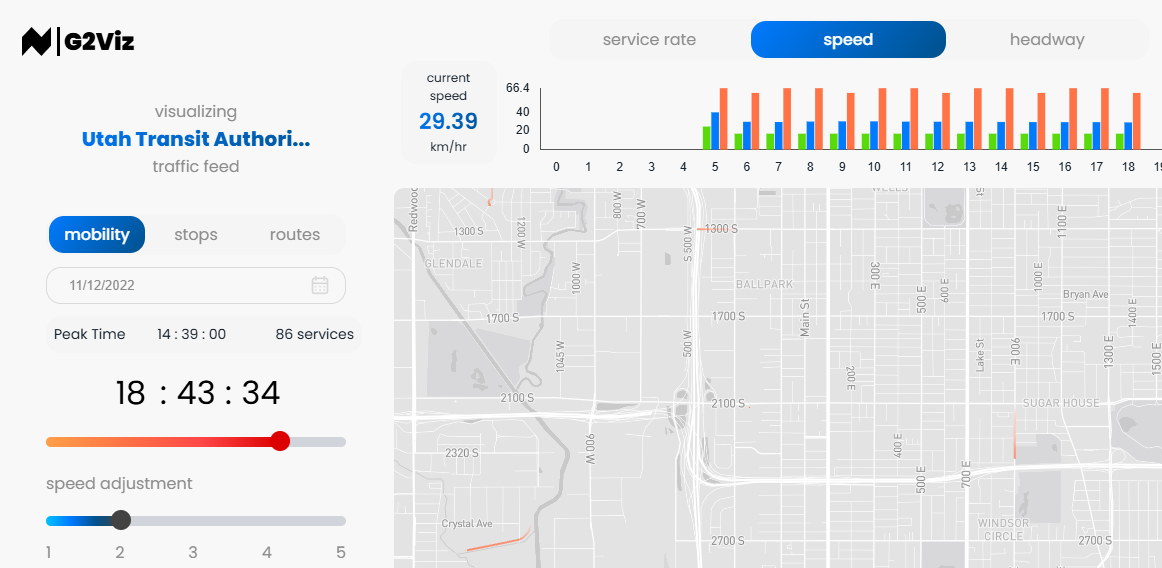
\includegraphics[width=0.9\textwidth]{figures/g2viz.png}
    \caption{G2VIZ nimelises tööriist, kus on näha ühissõidukite kohta statistikat. Joonise üleval on visualiseeritud on iga tunni kohta keskmine, maksimaalne ja minimaalne kiirus. Kaardil saab näha sõidukite liikumisi. Visualiseerida saab staatilisi andmeid (GTFS) ehk mitte reaalseid liikumisi.}
    \label{fig:sample}
\end{figure}

G2VIZ puhul on tegu väga lihtsasti kasutatava veebilehega, kuhu saab üles laadida GTFS formaadis kokkupakitud faili \cite{2024_pt_g2viz}. Veebilehe kasutamine on tasuta, kuid ühe piiranguna on seatud üleslaaditava faili suurus. Maksimaalne suurus on 10 MB, mis näiteks ei võimalda üles laadida Eesti ühistranspordiregistrist saadaolevat faili, kuna selle suurus on rohkem kui 10 MB. Tallinna transpordi lehelt\footnote{\url{https://transport.tallinn.ee/data/gtfs.zip}} allalaaditav fail on kuskil 6 MB suur, kuid selle üleslaadimisel annab lehekülg veateate. Autor on kontakteerunud veebilehe haldajaga, kuid pole vastust saanud.

Pärast vea parandamist oleks teoreetiliselt lehel võimalik näha analüütilisi tulemusi maksimaalsete, minimaalsete ja keskmiste kiiruste kohta tundide järgi. Seda küll mitte geograafilise asukohtade järgi, vaid liinigraafiku põhjal. See tähendab ka, et antud rakendus ei arvesta liinivõrgus juhtuda võivate ummikute, õnnetuste ja muu ootamatute olukordade põhjustatud liinigraafikust kõrvalekalletega.

\subsection{Pikas}

Pikase puhul on tegu ühistranspordi sõiduplaanide koostamise ja koordineerimise programmiga. Tallinnas võeti süsteem kasutusele aastal 1994 \cite{merakas_projects}. Süsteemil on ka mitmeid liinivõrku analüüsivaid võimalusi. Näiteks on joonisel \ref{fig:pikasLeedu} näha kui palju sõidukid sõidugraafikust kõrvale kaldusid (sinine joon). On näha ka võimalusi vaadelda kiirusi ja sõidule kulunud aega. 

\begin{figure}[h!]
    \centering
    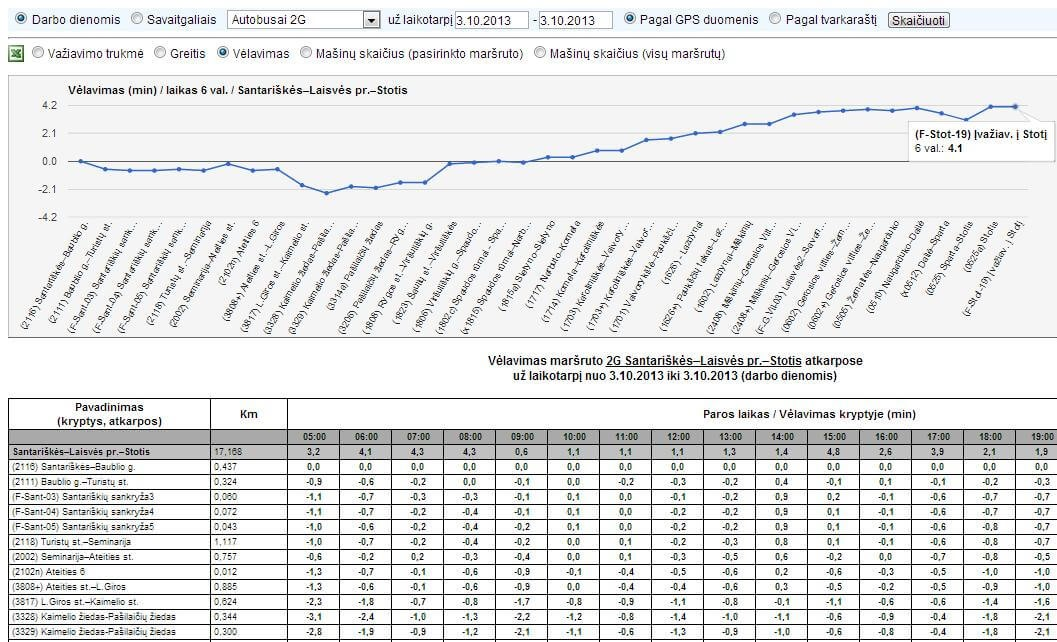
\includegraphics[width=1\textwidth]{figures/pikasLeedu.jpg}
    \caption{Analüütiline vaade Pikas süsteemis, kus on kuvatud bussiliini 2G hilinemine peatuste kaupa tööpäeval 3.10.2013 GPS andmete järgi on\cite{merakas_pikas}.}
    \label{fig:pikasLeedu}
\end{figure}


Pikas on osa ühistranspordi infosüsteemist (ÜTRIS), mida haldab Regionaal- ja Põllumajandusministeerium. Riigil ja Tallinna Linnatranspordil (TLT) on mõlemal oma Pikas nimeline süsteem. Aastal 2017 tehtud analüüsi käigus toodi välja, et süsteemil oli mõningaid puudusi. Näiteks olid andmed kahe süsteemi vahel dubleeritud ja liinivõrgu muudatused tuli ühest süsteemist teise käsitsi tõsta. See võttis väga palju aega, olenevalt muudatuste arvust võis kuluda 6 kuni 30 tundi. Toodi ka välja, et puudus arendus- ja hooldusleping tarkvara loonud firmaga, mis tähendas, et süsteemi funktsioone ei saanud edasi arendada \cite{tallinn_infosusteem_2017}. 

Autor ei ole teadlik, kas linnale kuuluva tööriista analüütiline osa on töökorras arvestades, et arendustegevus on olnud puudulik. Eeldades, et analüütiline süsteem on töökorras, siis autori arvamusel võiks taolised andmed olla avalikud. Kuna autori hinnangul on vähetõenäoline, et linn seda lähiajal teeks, siis proovitakse siin töös osaliselt seda teha. Küll mitte samamoodi, vaid pigem interaktiivse kaardirakendusena.

\subsection{Reisiplaneerijad}

Eestis on mitmeid reisiplaneerijaid, mis võimaldavad kasutajal näha ühistranspordi sõidukite liikumisi reaalajas. 

\begin{figure}[h!]
    \centering
    \begin{subfigure}{0.45\textwidth}
        \centering
        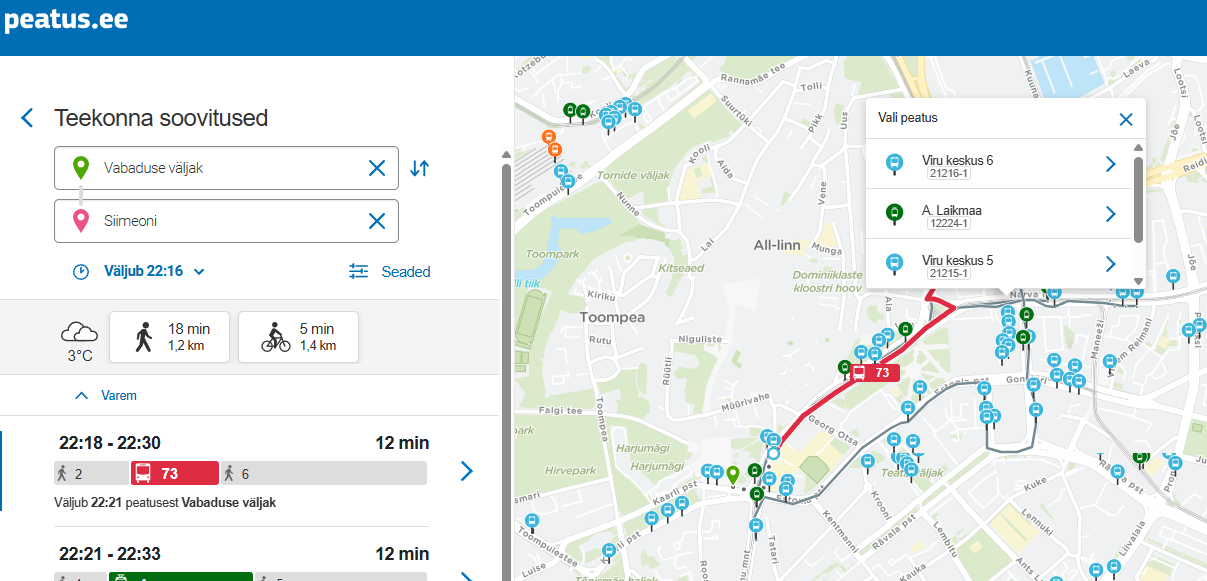
\includegraphics[width=\textwidth]{figures/peatus.png}
        \caption{}
        \label{fig:Peatus.ee}
    \end{subfigure}
    \hfill
    \begin{subfigure}{0.45\textwidth}
        \centering
        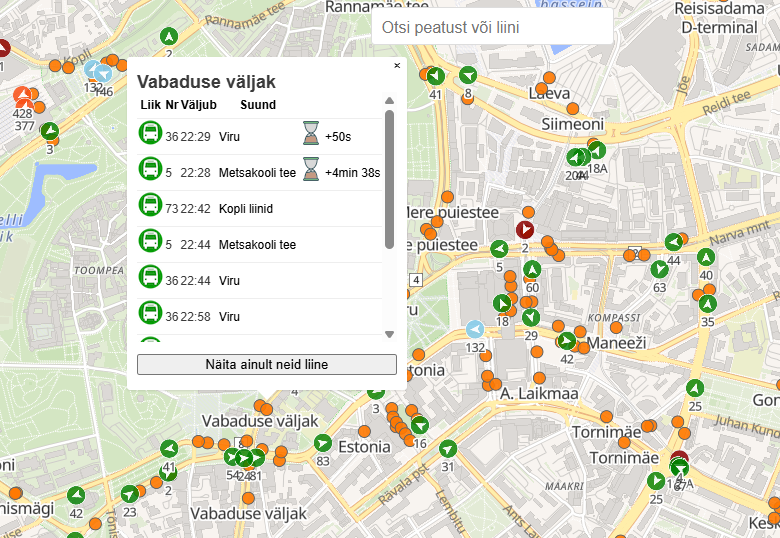
\includegraphics[width=\textwidth]{figures/gis.png}
        \caption{}
        \label{fig:https://gis.ee/tallinn/}
    \end{subfigure}
    \caption{Tallinnas avalikult kättesaadavad reisiplaneerijad (a) \url{https://web.peatus.ee/} ja (b) \url{https://gis.ee/tallinn/}.}
    \label{fig:combined}
\end{figure}

Joonisel \ref{fig:Peatus.ee} olev veebileht  on lihtsasti kasutatav reisiplaaneerija, mis peale liini valimist näitab sõidukite reaalajas liikumist. Ühe lisavõimalusena näeb seal ka maakonnaliinidel sõitvate busside liikumist. Veebileht saab oma andmed eeltoodud Pikase süsteemist \cite{tallinn_infosusteem_2017}.


Joonisel \ref{fig:https://gis.ee/tallinn/} olev veebileht on samuti reisiplaneerija, kuid seal on kohe avavaates olemas ka üle terve linna reaalajas liikuvad sõidukid ja iga peatuse juures on lisainfo hilinemiste kohta.

Tallinnal on ka eraldi veebileht \footnote{\url{https://transport.tallinn.ee/}}, kust saab vaadelda reaalajas väljumisi. 

Kõikide reisiplaneerijate puhul on puuduseks see, et rakendused ei ole mõeldud mitte ühistranspordi võrgu analüüsimiseks, vaid hetkeliseks vaatluseks.


\section{GNSS andmete ebatäpsus}

GNSS (\textit{Global Navigation Satellite System}) on ühine sõna erinevatele sateliitide süsteemidele, mis pakuvad globaalset positsioneerimist. Enim tuntud on Galileo, GPS (\textit{Global Positioning System}), GLONASS ja BeiDou \cite{euspa_gnss}. 

USA kosmoseväe andmetel jääb nende GPS asukohaandmete vertikaalne täpsus 95\% juhtudel alla 13m ja horisontaalne täpsus 95\% juhtudel alla 8m. Vertikaalsihi all peetakse siin silmas kõrgust ja horisontaalsihi all laius- ja pikkuskraade \cite{GPS_performance}. 
GPS asukohad võivad erineda reaalsest asukohast mitmel põhjusel:
\begin{itemize}
    \item Sateliidi signaal on blokeeritud hoonete tõttu.
    \item GPS seade on maa all või siseruumides.
    \item Signaal peegeldus seinast.
\end{itemize}

\section{Sarnased tööd}

Aastal 2016  Tampere Ülikooli poolt tehtud põhjaliku uuringu tulemusel valmis andmepõhine ühistranspordi graafik \cite{Syrjarinne2015}. Selleks leiti graafiku hilinemised esialgsest sõidugraafikust ja parandati vajalikud kohad. Töös toodi välja, kuidas alles ei hoitud mitte kõiki andmeid, vaid sissetulevad andmed töödeldi ja alles hoiti vaid info, mis oli seotud peatustega. Peatusesse saabumise info saadi selliselt, et otsiti mingi sõiduki teekonna kõiki punkte, mis peatuse raadiusse R jäid. Ajaliselt kõige varasem punkt oli peatusesse saabumise aeg ja kõige hilisem punkt sealt väljumise aeg. Töös koguti asukohti kord sekundis. Oma olemuselt koguti andmeid 30 korda tihedamalt kui antud töös, see tähendab, et osad tulemused on siinses töös üldisemad.

Teatud tööde puhul on analüüsitud ainult staatilisi ühistranspordi andmeid. Näiteks 2023 aastal avaldatud teadusartiklis \cite{2024_pt_g2viz} analüüsiti gtfs2gps teegi kasutamise võimalusi. Sisult tähendas see peatuste asukohtade, ajagraafikute ja muu mittereaaalajaandmete analüüsi tööriista abil.

Lisaks valmis 2024 aasta detsembris ka gps2gtfs teek, mis võtab sisse korrastamata gps andmed ja väljastab GTFS formaadis reaalajaandmed. Vastavalt teegi loonud autorite andmetele on tegu esimese taolise teegiga \cite{GPS_2_GTFS}. Andmete ühesuguseks muutmine on väga oluline protsess, kuna see võimaldab paremini luua vastavatele andmetele loodud tööriistu. Teoorias aitaks näiteks luua standartidele paremini vastava andmebaasi, mida oleks hõplsam jagada ja teistel kasutada. Kuid isegi teegi olemasolul jäävad õhku küsimused andmete kogumisest, hoiustamisest ning visualiseerimisest.

Tallinna puhul on vähe teada tehtud töödest, kuid nii Dago Antovi kui põgusalt linnaga suheldes, siis mõlemal on suheldes olnud huvi ühistransporti analüüsivate tööriistade järgi.

\section{Ühistranspordi kiirused maailmas}

Pea igas maailma linnas on mingil tasemel olemas ühistranspordi võrgustik. Mõnes linnas kiiremini  ja mõnes aeglasemini liikuv. Rootsi linnade ühistransporti uurivas töös leiti, et sealsetes linnades on ühistranspordi kiirused muude Euroopa ja maailma linnadega võrreldes suuremad \cite{urbansci3010025}. 

\begin{longtable}{|l|c|c|c|c|c|}
\caption{Ühistranspordi keskmised kiirused valitud piirkondades (km/h) \cite{rigas_satiksme_passengers_2019}, \cite{urbansci3010025}.}
\label{tab:maailmaKiirused}\\ \hline % Sets a label for the table and starts the table with a horizontal line
\textbf{Piirkond} & \textbf{Stockholm} & \textbf{Rootsi}  & \textbf{Riia} & \textbf{Euroopa} \\ \hline
Aasta & 2015 & 2015 & 2019 & 2005 \\
\hline
Busside keskmine kiirus (km/h) & 24,8 & 27,1 & 20,5 & 21,9 \\ \hline
Trammide keskmine kiirus (km/h) &   &   & 15,9  & 16,9 \\ \hline
Kergraudtee keskmine kiirus (km/h) & 30,5 &   &   & 25,9 \\ \hline
Metroo keskmine kiirus (km/h) & 34,0 & 34,0 &    & 33,5 \\ \hline
Lähirongide keskmine kiirus (km/h) & 56,3 & 71,5 &    & 52,1 \\ \hline
Trollide keskmine kiirus (km/h) &   &   & 15,6  &   \\
\hline
\end{longtable}

Rootsi puhul on leitud, et ühistransport on Malmös keskmiselt 14\% kiirem, kui sealne autoliiklus. Stockholmis seevastu on 9\% aeglasem, ning Rootsi linnades üldiselt on ühistransport keskmiselt 2\% aeglasem \cite{urbansci3010025}. Antud töös leitud Tallinna kiirused on leitavad tulemuste alt. Kuid siiski ei saa ainult suurt sõidukite kiirust pidada hea ühistranspordi tunnuseks. Järgnevalt on toodud mõned probleemsed näited:
\begin{itemize}
    \item Hõre linn / valglinnastunud linn - kiirused on suured, aga vahemaad on veelgi suuremad ja sihtpunkti jõudmine võtab rohkelt aega.
    \item Ühistransport on kiire, aga ühistranspordivõrk katab väikse osa linnast ehk peatusi on hõredalt.
    \item Ühistranspordi võrk on väga käänuline. Kõrvalistel teedel saavutatakse küll kõrged kiirused, aga sihtpunktide poole liigutakse linnulennult aeglaselt.
\end{itemize}
Sellegipoolest on keskmine kiirus üldiselt üks hea näitaja ühistranspordi kvaliteedi hindamiseks ja teiste sarnaste linnadega võrdlemiseks.






\chapter{Metoodika}\label{chapter:method}

Töö planeerimisel ei olnud esialgu selge, kuidas täpselt töö valmima peaks. Autoril puudus nii otsene kui kaudne kokkupuude suurte andmebaaside loomise ja haldamisega. Seetõttu kaasnes tööga palju katseid ja ka läbikukkumisi. Siin peatükkis on kirjeldatud, kuidas jõuti lõpptulemuseni.

\section{Lahenduse arhitektuur} %This creates a new subsection titled 
\begin{figure}[h!]
    \centering
    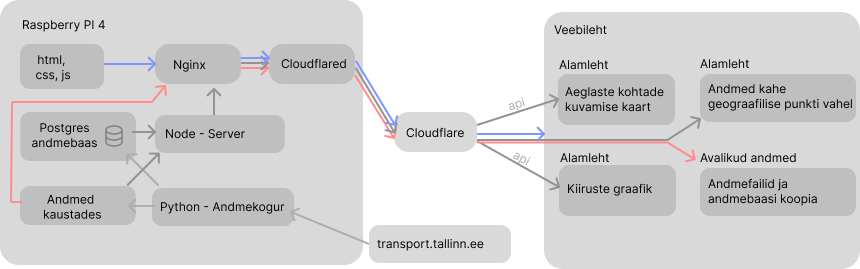
\includegraphics[width=0.95\textwidth]{figures/struktuur.png}
    \caption{Arhitektuuriline lahendus.}
    \label{fig:Struktuur}
\end{figure}

Joonisel \ref{fig:Struktuur} on näha, kuidas andmed kogutakse \url{transport.tallinn.ee} kaudu. Andmete kogumiseks on kirjutatud Pythoni skript. Geograafilised asukohad salvestatakse andmebaasi, muud andmed salvestatakse kaustadesse. Kui kasutaja avab veebilehe, siis turvalisuse tagamiseks on kasutusel Cloudflare nimeline teenus. Kogu suhtlus käib läbi Cloudflare serveri, see tähendab, et Raspberry Pi  IP-aadress ei ole avalik. Lokaalselt on kasutusel Node server, mis teeb päringuid PostgreSQL andmebaasi pihta.

\section{Andmete päritolu}


Enne andmete kogumist tuli kaardistada kohad, kust andmeid on võimalik koguda. Selleks uuriti, kust saab andmed Tallinna ühistranspordi leht \footnote{\url{https://transport.tallinn.ee/}} ja vaadati üldiselt internetis ringi, et kas leidub veel kohti.
Tõenäoliselt ei ole Tabel \ref{tab:andmeteAsukohad} tulem täielik.

\begin{longtable}[hp]{|p{5cm}|p{4cm}|p{2cm}|p{2cm}|} % Begins a longtable with three columns, defining specific widths for each column
	\caption{Kohad kust andmeid koguda.} % Provides a caption for the table, italicizing the text
	\label{tab:andmeteAsukohad}\\ \hline % Sets a label for the table and starts the table with a horizontal line
	\textbf{URL} &  \textbf{Andmeliik} & \textbf{Andmetüüp} & \textbf{Töös kogutud}  \\ % Table header with bold text
	\hline % Adds a horizontal line after the header
	\endfirsthead % Marks the end of the header for the first page of the table
	\multicolumn{3}{l} % Merges three columns for the continuation note
	{\tablename\ \thetable\ -- \textit{Jätkub...}} \\ % Creates a continuation note with italicized text
	\hline
	\textbf{URL} &  \textbf{Andmeliik} & \textbf{Andmetüüp} & \textbf{Töös kogutud}   \\  % Table header for continued pages, with bold text
	\hline
	\endhead % Marks the end of the header for all pages after the first
	\hline \multicolumn{3}{l}{\textit{Jätkub...}} \\ % Adds a note at the end of the table for continued pages
	\endfoot % Marks the end of the table body
	\hline
	\endlastfoot % Marks the end of the table for the last page
 \url{https://transport.tallinn.ee/gps.txt} & Reaalajas asukohad & CSV & Ei\\ \hline 
\url{https://transport.tallinn.ee/ readfile.php?name=gps.txt} & Reaalajas asukohad & CSV & Jah, iga 30s tagant\\ \hline
\url{https://gis.ee/tallinn/gps.php} & Reaalajas asukohad & JSON & Ei\\ \hline

 \url{https://transport.tallinn.ee/data/tallinna-linn\_bus\_18.txt} & Ühissõidukite marsruudid (iga marsruut eraldi) & TXT & Jah, kord päevas kell 04:00\\
\hline 
\url{https://transport.tallinn.ee/data/routes.txt} & Ühissõidukite sõiduplaanid & TXT &Jah, kord päevas kell 04:00\\
\hline 
\url{https://transport.tallinn.ee/data/stops.xml} & Peatuste asukohad & XML & Jah, kord päevas kell 04:00\\
\hline 
\url{https://transport.tallinn.ee/tabloconfig2021.php} & Ebaselge, kuid paistab kuvavat infot juhul kui väljumist ei toimu, kuid mitte alati & JSON & Ei\\
\hline
\url{https://transport.tallinn.ee/interruptions.json} & Ootamatud tõrked & JSON & Jah, iga 5 minuti tagant\\
\hline 
\url{https://transport.tallinn.ee/announcements.json} & Teadaanded & JSON & Jah, kord päevas kell 04:00\\
\hline
\url{https://transport.tallinn.ee/data/gtfs.zip} & Tallinna GTFS formaadis andmed  & ZIP & Jah, kord päevas alates aprill 2025\\
\hline
\url{https://www.peatus.ee/gtfs/gtfs.zip} & Eesti GTFS formaadis andmed  & ZIP & Ei\\
\hline
\end{longtable}
\newpage
Antud tabeli puhul on oluline märkida, et kohad, kust andmeid koguti, muutusid ajas. Seda seetõttu, kuna töö käigus avastati uusi kohti. Näiteks 2025 kevadel leiti koht, kust laadida Tallinnat puudutav info ühest kohast ühe failina \footnote{\url{https://transport.tallinn.ee/data/gfts.zip}}. Kogu Eesti andmeid ei kogutud, kuna see polnud töö eesmärk. Reaalaajandmete puhul oli valikus mitu kohta, kust andmeid saada, kuid lõpuks jäädi praeguse lahenduse juurde, kuna sealt saadavatel andmetel oli lisatulp sihtkoha infoga.

Kuigi väiksed muudatused toimusid, siis lõplikult kogutakse järgmist infot:
\begin{enumerate}
    \item Reaalaajaandmed: aeg, liin, sõidukitüüp, asukoht, sihtpunkt, sõiduki identifikaator, suund.
    \item Teadaanded: liinide ja sõidugraafikute muudatused.
    \item Ootamatud tõrked: info tõrgete kohta.
    \item GTFS: peatuste asukohad, marsruudid, ajagraafikud jne.
    
\end{enumerate}



\section{Raspberry Pi serverina} % This creates a new section with the title "First Section of the First Chapter."
Raspberry Pi 4 on ühendatud 1-terabaidise kõvakettaga, mõlemat on näha Joonisel \ref{fig:RaspberryPi}. Seadistamiseks on kasutatud 64 GB mälukaarti, millele paigaldati \textit{Raspberry Pi OS Lite (64-bit)} operatsioonisüsteem.
Serveri töökindluse tagamiseks on seadistatud valvetimer (\textit{watchdog timer}), mis taaskäivitab süsteemi, kui see peaks kokku jooksma. Käivituse järel toimub automaatselt kõvakettaga ühendamine ja andmekogumise protsessi käivitamine.

\begin{figure}[h!]
    \centering
    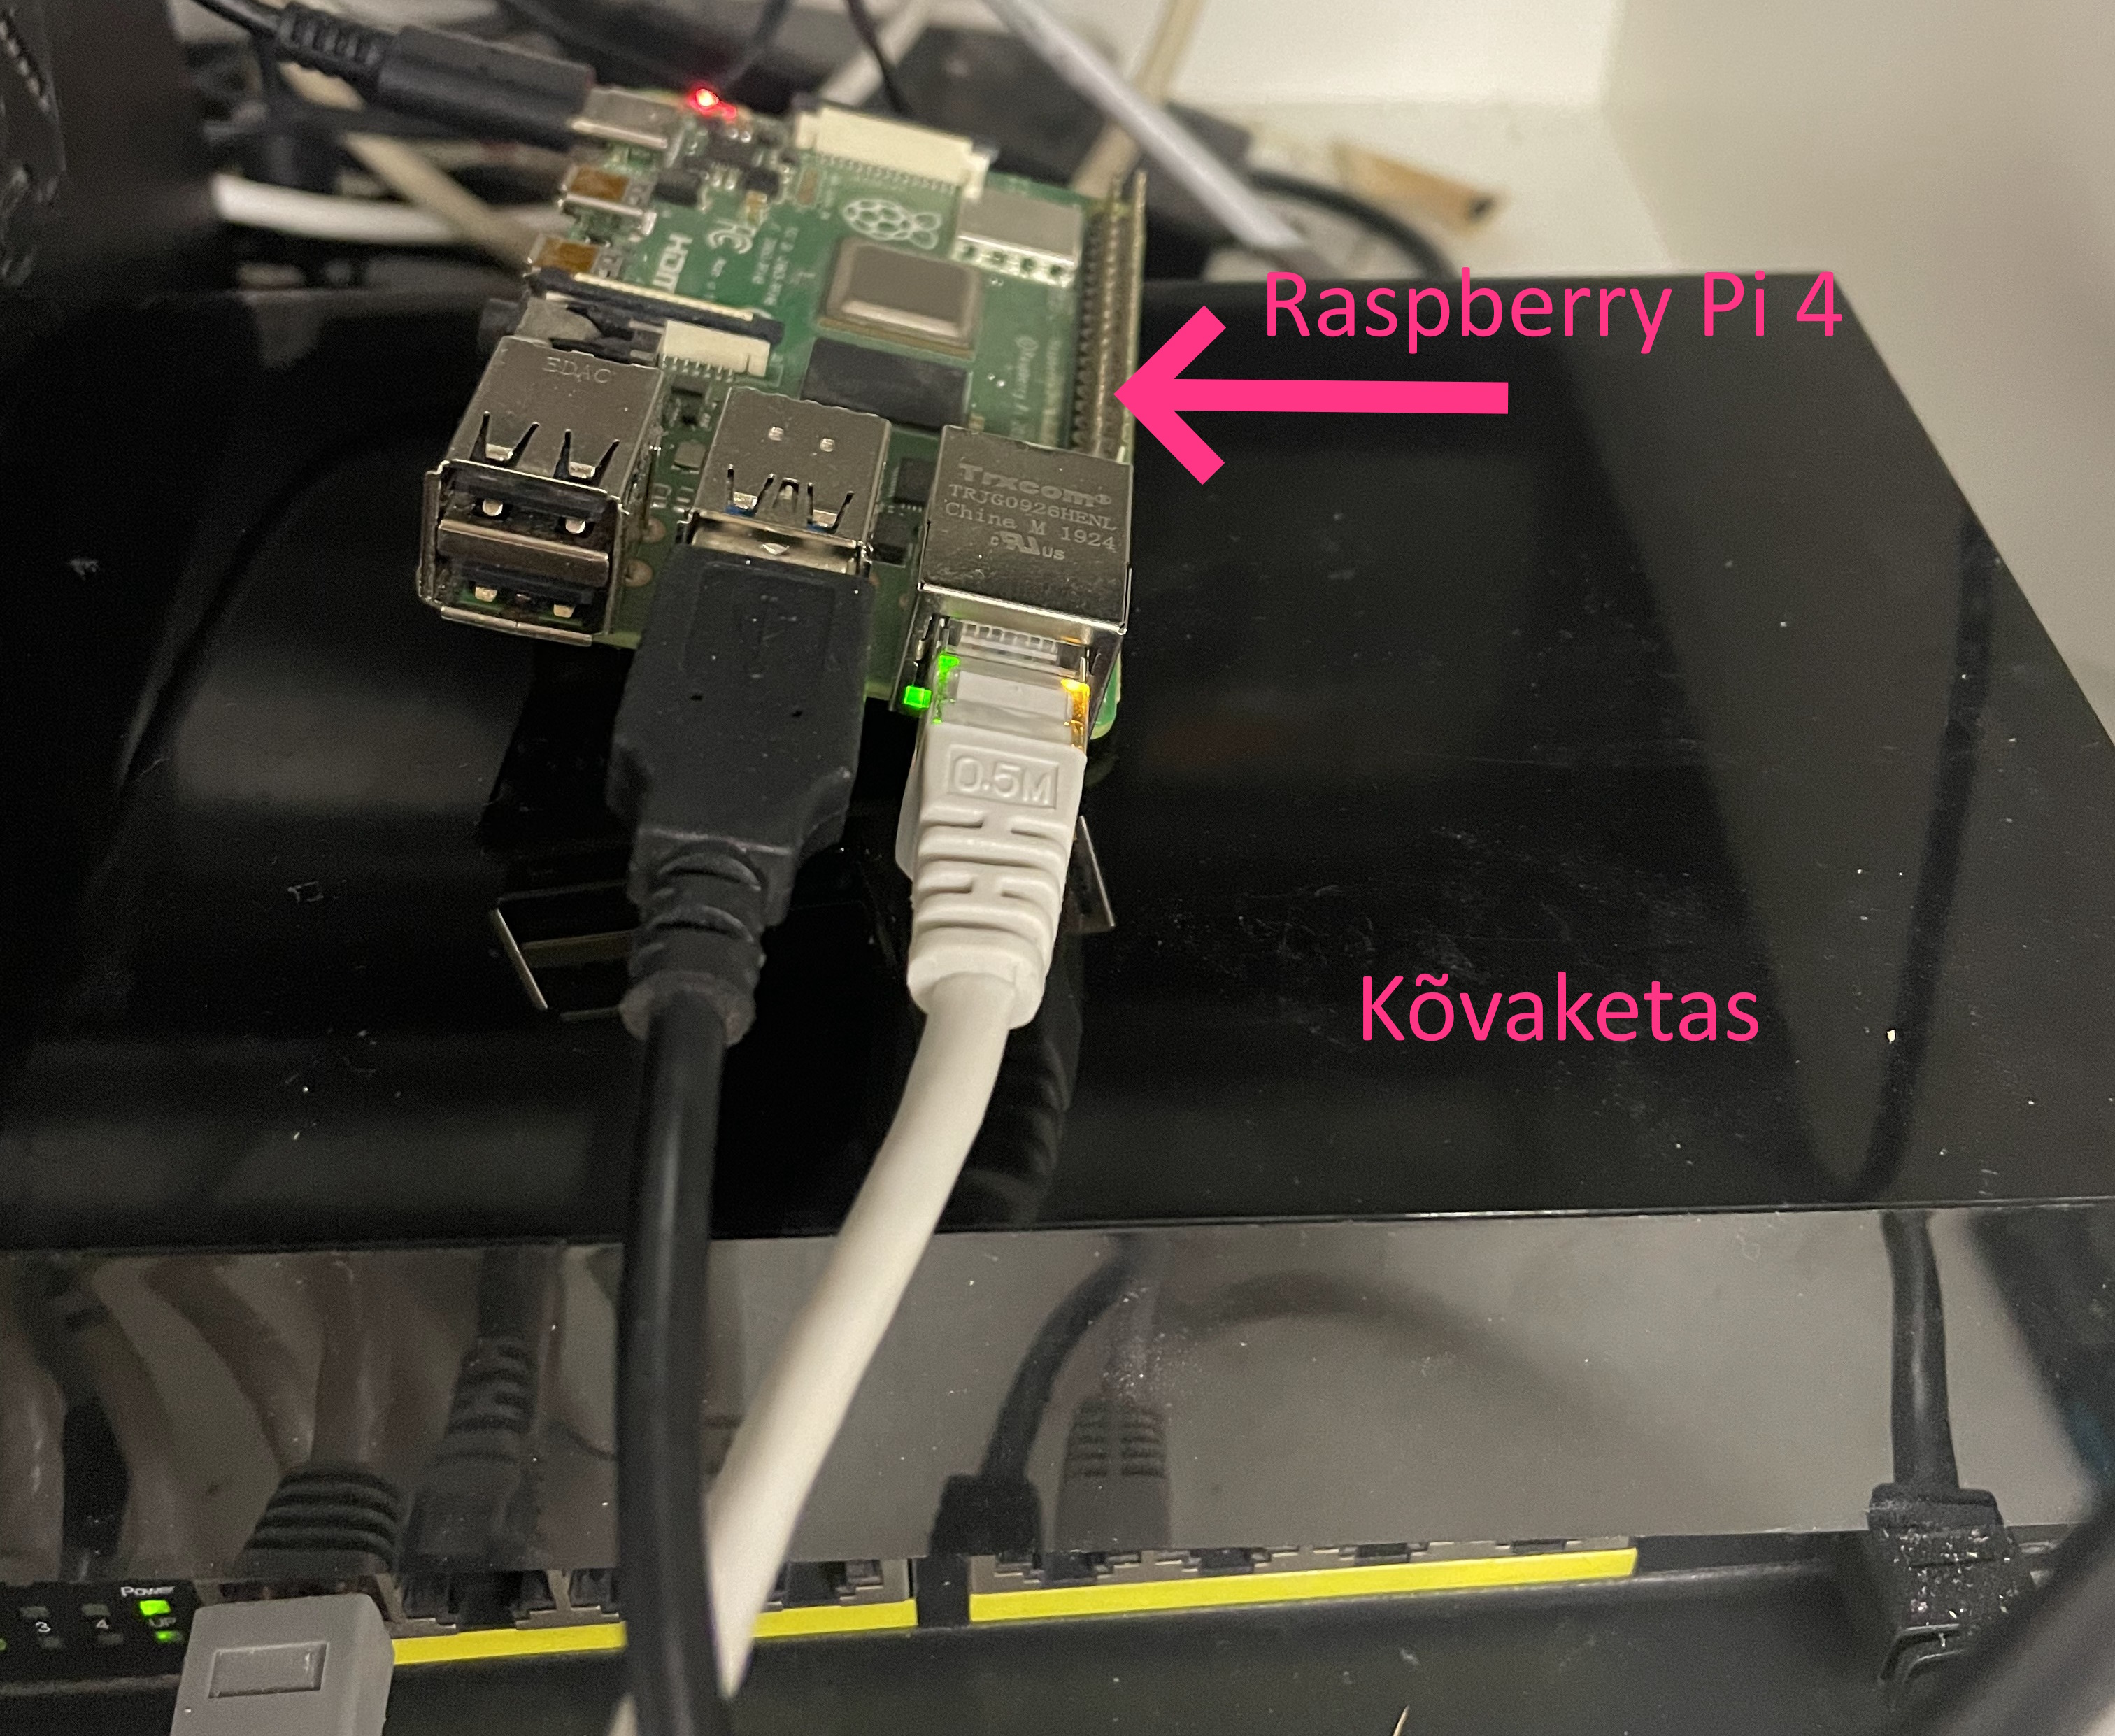
\includegraphics[width=0.45\textwidth]{figures/RaspberryPi.jpg}
    \caption{Rasberry Pi 4 ja kõvaketas autori kodus.}
    \label{fig:RaspberryPi}
\end{figure}

Raspberry Pi 4 ja kõvaketas valiti töö jaoks, kuna mõlemad olid autoril enne tööga alustamist juba olemas ja rahaliste väljaminekute vältimiseks otsustati neid ka kasutada. Teiste variantidena kaaluti lauaarvuti kasutamist, kuid oma suure suuruse ja müra tõttu tundus see ebapraktiline. Raspberry Pi oli ilma mürata ning selle sai paigutada kitsasse kappi. Kolmanda variandina kaaluti virtuaalse privaatse serveri kasutamist. Kuid nende puhul on üldjuhul tegu tasuliste teenustega \cite{Hetzner2025}, millel on rangemad piirangud kui enda hallataval serveril. Soov omada täielikku kontrolli serveri üle, hind ja eksperimenteerimise lihtsustamine jätsid pilvepõhise serveri valikust välja.



\section{Andmete kogumise skript} % This creates a new section with the title "First Section of the First Chapter."
Reaalaajaandmete kogumiseks on kirjutatud Pythonis skript, mida haldab \textit{systemd} ja mis käivitatakse \textit{systemctl} käsureatööriista abil teenusena. See võimaldab skripti automaatset käivitamist, tõrgete korral taaskäivitamist ning logide jälgimist.

Staatilisi andmeid kogutakse iga päev kell 04:00. Esialgu koguti andmeid selliselt nagu \url{transport.tallinn.ee} oma enda veebilehe siseseid päringuid tegi, mis tähendas, et osad andmed olid ebastandartsel kujul ja inimesele raskesti arusaadavad. Kõige suuremaid raskusi põhjustas autorile ajagraafiku failist \footnote{\url{https://tallinn.simplytobo.eu/transport_data/transport_data/bus_times_data/2025-06-04/routes.txt}} arusaamine, ning autor ei suutnudki seda lõpikult teha. See muutis teisele uurimusküsimusele ("Kui suured on liinil sõitvate sõidukite hilinemised?") vastuse leidmise väga ajanõudvaks. Alles töö lõpus leiti, et samal leheküljel eksisteeris ka paremini arusaadav fail.
 
Töö lõpus leiti, et \url{transport.tallinn.ee} lehel on olemas GTFS formaadis koht, kust saab heal kujul andmeid, sealhulgas ajagraafikuid. Autor lisas GTFS andmete kogumise loogika.  Selleks tehakse igal hommikul päring päise (\textit{header}) küsimiseks. Kui päises on rida (\textit{Last-Modified}), mis kirjeldab millal viimati andmeid muudetud, on vahepeal uuenenud, siis tehakse uus päring ja laetakse andmed päriselt alla. GTFS fail on  pigem väike (alla 10 MB), kuid hea tava on ikkagi laadida ainult siis, kui vajadus.

Iga päev saadab skript välja teate autorile sotsiaalmeedia platvormile Discord. Sõnum sisaldab infot selle kohta, kas andmete kogumine endiselt töötab ja kui palju andmeid eelmine päev salvestati. Juhul kui andmete salvestamine mingil põhjusel ebaõnnestub, siis selle kohta saadetakse koheselt veateade. See võimaldas autoril jälgida toimuvat telefonist ja mitmed vead avastati just nii.
 
\section{Andmete hoiustamine}

Andmete hoiustamiseks katsetati mitut viisi. Esialgu koguti kõiki andmeid kaustadesse. Andmed jaotati esialgu nende tüübi (6 kausta), siis kuupäeva (365 kausta aastas) ja siis salvestati fail selliselt, et kellaaeg oli nimeks. Antud viis töötas hästi, kui andmeid oli vähe. 

Reaalajaandmeid hakkas aja jooksul kogunema nii palju, et mitme päeva analüüsimine muutus väga aeglaseks. Samuti tuli kõik andmetega ümberkäivad funktsioonid nullist kirjutada. Pythoniga muutus see kiirelt liiga aeglaseks ja raskesti hallatavaks. Autor proovis kasutada komplileeritud keelt nagu Go ja kuigi seal oli andmetega ümberkäimine kordades kiirem, oli see endiselt raskesti hallatav. 

Juba 2024. sügisel valiti proovimiseks SQLite andmebaas. Seda seetõttu, kuna tol hetkel usuti, et selle jõudlusest piisab. Katsetuste käigus selgus, et andmete andmebaasi saamine on väga ajakulukas ning päringute tegemine on kohati aeglasem kui otse kaustast võtmine. Prooviti mitmeid optimeerimise viise. Näiteks andmebaasi kuu suurusteks tükkideks jagamist, ajatulba indekseerimist, andmebaasi tõstmist võimsama arvuti peale, kuid lõpuks muutus andmebaasiga ümberkäimine liialt ajakulukaks. Autor otsis seejärel uut viisi andmete hoiustamiseks.

Juhendaja soovitusel uuriti täpsemalt aegrea andmebaaside võimalusi. Valikuvariantide all olid InfluxDB, Prometheus, Graphite ja TimescaleDB. Valiku tegemine oli raske, kuid lõpuks otsustati TimescaleDB kasuks. Seda nimelt seetõttu, et tegu on PostgreSQL andmebaasi lisaga. PostgreSQL on aga üks kõige populaarsemaid andmebaasihaldussüsteeme \cite{dbengines_ranking}. See tähendab head dokumentatsiooni, kuidas asju teha. Täpsema uurimise tulemusena avastati ka võimalus ühildada omavahel TimescaledDB ja PostGIS. PostGIS võimaldab teha geograafilisi päringud väga kiiresti ning sobis seeläbi hästi töös kasutatavate andmete visualiseerimiseks.

\subsection{Andmemaht}

Töö algul moodustasid reaalajaandmed 98\% andmemahust. JSON kujul andmeid kogunes päevas 80 - 120 MB, nädalas 700 MB, kuus 3 GB ja aastas 36 GB. Seevastu muid andmeid kogunes alla 2 MB päevas. 27. detsember 2024 ehk 6 kuud peale andmete kogumist oli kõikide kaustade kogusuurus 18,4 GB. Mingil hetkel nähti võimalust koguda andmeid CSV kujul ehk ilma JSON failis ebavajaliku lisainfota. Selliselt kogunes päevas 20 - 30 MB andmeid päevas. See tähendanuks, et kuue kuuga oleks kogunenud 4,2 GB andmeid, mis on pea 80\% vähem. See oli juba päris hea, kuid päringute kiirused olid kaustades andmete puhul endiselt aeglased. Seetõttu liiguti järgmise viisi juurde.

Vahepeal katsetati SQLite andmebaasi võimalusi, kuid andmemahud olid seal sama suured ja suuremadki kui samapalju andmeid JSON kujul kaustades. 

Lõpuks jõuti TimescaleDB juurde ja leiti viis seal andmeid optimaalsemalt hoiustada.  Optimeerimise käigus muutus andmebaasi suurus 26 GB pealt 2,8 GB peale (9 kuu andmed). Oma olemuselt seati reaalajaandmete hoiustamisel sisse reegel, et peale seitset päeva andmebaasis olemist muudetakse reapõhine andmebaas tulbapõhiseks ja andmete hoiustamine muudetakse optimaalsemaks \cite{timescale_hypercore}. Selle tulemusel oli andmebaasi nüüd võimalik jagada ja internetist alla laadida mõistliku aja piires\footnote{\url{https://tallinn.simplytobo.eu/transport_data/transport_data/realtime_database_copy/}}. Vahepeal katsetati kiiruse lisatulba lisamisega andmebaasile, mille käigus loodi uus andmebaas nullist, ning tehti samad eelpool tehtud käsud. Peale seda oli andmebaas 2,7 GB suur ja sisaldas 10 kuu andmeid. Võrreldes JSON kujul andmete hoiustamisega oli lõplik tulemus 90\% optimaalsem.

Kaustades andmete probleem oli ka nendest koopia tegemise ja jagamise aeglus. Ühe kuu andmete allalaadimine võttis kuskil 15 minutit ja 10 kuu puhul tuli arvestada 3 tunniga. TimescaleDB andmebaasiga  võttis aga 10 kuu kohta koopiafaili tegemine 12 minutit ja selle faili allalaadimine võttis 2 minutit. Allalaadimine muutus 99\% kiiremaks (3 tunni pealt 2 minuti peale).

\section{Kiiruste arvutamine}

Kuigi kohad, kus kiirusi arvutati, on ajas muutunud, on seda üldiselt alati samamoodi tehtud. Võetakse kaks järjestikku olevat andmerida ja leitakse nendevaheline vahemaa ja aeg. Seda teades on lihtne leida keskmine kiirus selle 30 sekundi vältel (andmeid kogutakse iga 30 sekundi tagant). Töö lõpupoole hakkas kasutuses olema Joonisel \ref{fig:kiirusteSQLskript} näidatud skript. Siiski on siin ebatäpsus, kuna vastavalt kasutaja soovidele luuakse dünaamiline päring ning lisaks on teatud kohtades välja võetud depood ja lõpppeatustes seismised. Samuti on kohati võimalik välja filtreerida tulemusi, mis on peatuste lähedal (Joonis \ref{fig:Kiirustekaart}).  

\begin{figure}[h!]
    \centering
    \scriptsize
\begin{lstlisting}
WITH speed_data AS (
    SELECT
        datetime,
        geom,
        LEAD(geom) OVER (PARTITION BY type,line,vehicle_idORDER BY datetime)
        AS next_point,
        LEAD(datetime) OVER (PARTITION BY type, line,vehicle_id ORDER BY datetime)
        AS next_time
    FROM realtimedata
),segment_data AS (
    SELECT
        EXTRACT(EPOCH FROM (next_time - datetime)) 
        AS time_diff_seconds, 
        ST_Distance(geom::GEOGRAPHY, next_point::GEOGRAPHY) 
        AS distance_meters
    FROM speed_data
    WHERE next_point IS NOT NULL)
SELECT 
    (distance_meters / time_diff_seconds) * 3.6 
    AS speed_kmh 
FROM segment_data;
\end{lstlisting}
\caption{SQL päring sõiduki kiiruse arvutamiseks.}
\label{fig:kiirusteSQLskript}
\end{figure}

\section{Andmete visualiseerimine}

Alguses kogunes päevas 2880 reaalajaandmete faili kaustadesse ning andmete visualiseerimiseks tehti skript, mis pani kõik andmed ühte faili ja pakkis kokku. Hiljem skripti kiirust mõõtes selgus, et ühe päeva andmete salvestamiseks kulus 12 minutit. Seejärel veebileht sai teha päringu ja päeva andmed serverist alla laadida. Veebileht kasutab kaardi kuvamiseks Leaflet teeki \cite{leafletjs}. Antud kaardile lisati seejärel saadud asukohtade koordinaadid. Võimalik oli liikuda ajas edasi ja tagasi ning näha sõidukite liikumisi. Tegu oli lihtsa lehega. Edasiarenduste tegemine oli keeruline, kuna andmetöötlus oli aeganõudev ning halvasti hallatav. Sellegipoolest loodi Joonisel \ref{fig:Kiirustekaart} näha olev leht. Veebilehel kirjutati kood, mis grupeerib aegread aja asemel liini, tüübi ja sõiduki identifikaatori järgi. Seejärel olid andmed korrastatud sõidetud marsruutide järgi. Seda sai visualiseerida graafikul. Kuna bussikiirused kõiguvad väga palju ja andmeid on palju, siis paremaks kuvamiseks on iga andmepunkt nelja eelmise punkti keskmine. Kuigi muu eeltoodu ei ole enam kasutuses, siis see on endiselt alles.

Andmete TimescaleDB andmebaasi tõstmisel tekkis vajadus serveri järele, mis võtaks vastu veebilehelt tulevad päringud, teeks päringu andmebaasi pihta ja tagastaks andmed. See muutis ka andmetöötluse loogikat. Nüüd toimus kõik SQL päringute kaudu. Endiselt leiti vahemaa kahe punkti vahel ja kulunud aeg. PostGIS andmebaasi laiendus muutis vahemaa leidmise eriti lihtsaks ja kiireks. Samuti võimaldas see välja lõigata liini otstes ja depoodes seismised.

Ühe päeva andmete pärimine võttis nüüd aega 0,5 kuni 1,5 sekundit (enne 12 minutit). Võrreldes esialgse skriptiga muutis see veebilehe arenduse 99,9\% kiiremaks. Mitmesajarealise skripti asemel oli nüüd paarikümnerealine SQL kood (Joonis \ref{fig:kiirusteSQLskript}), veebilehele saadeti vaid vajalikud andmed ning üldine koodi hallatavus paranes oluliselt.

\section{Andmete kvaliteet}

GNSS andmete kvaliteeti mõjutab asjaolu, et andmete pärimisel ei ole antud kaasa kellaaega, millal sõiduk oma asukoha teada annab. See tähendab, et aeg ja ruum ei lähe kunagi kokku. Kuid kuna andmete kogumine toimub alati sama intervalliga (30s), siis pika aja vältel on viga võrdlemisi sarnane ja muutub ebaolulisemaks. Samuti ei ole oluline kiiruste analüüsiks täpsed asukohad, vaid asukoha ja aja muut. 

Keerulisem on lugu GNSS asukohtadega, kuna need ei pruugi näidata õiget kohta kaardil. Seda visualiseerib ka allolev joonis.

\begin{figure}[H] % h-here, if possible; H-here, definitely; t-top of the page; b-bottom of the page; p-page of floats
    \centering
    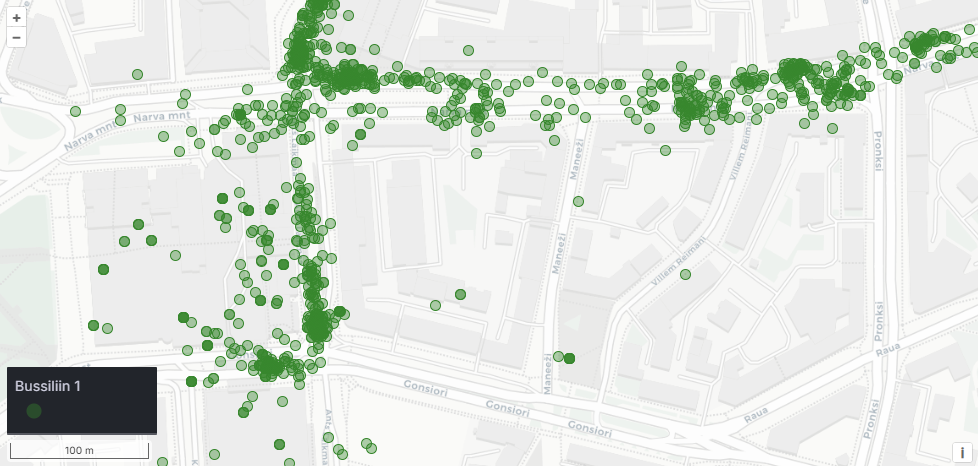
\includegraphics[width=.8\textwidth]{figures/gpsvead.png} % Includes an image from the specified path, setting the width to 50% of the text width
    \caption{Veaga asukohad Kesklinnas.} % Provides a caption for the figure, italicizing the text
    \label{fig:gpsnoise} % Sets a label for the figure to be referenced later 
\end{figure}

Joonisel \ref{fig:gpsnoise} on näha, et sõidukite asukohad võivad kohati näidata end majade peal ehk  kohtades, kuhu bussidel ligipääs puudub. Samuti on näha ebatäpseid mõõtmisi seoses Viru Keskuse maaaluse bussipeatusega. See raskendab täpsete mõõtmiste tegemist. Kuid sellegipoolest on müra sees võimalik näha, et enamus mõõtmisi jääb tänavavõrgustikule. Teatud meetoditega on võimalik andmete kvaliteeti tõsta. Näiteks kaardiga sobitamine (\textit{map matching}), kus sõidutee piiridest välja jäävad koordinaadid saab seostada olemasoleva lähimal oleva teega ja tõsta õigesse kohta, selleks on olemas omaette teegid nagu barefoot \cite{barefoot}. Iga päev kogutakse kokku ka liinide marsruudid ja seal ei lõigata kurve sirgeks. Maailmas on näiteid, kus on märgatud, et kui GNSS asukohad on teatud veaga, siis staatilised andmed nagu marsruut ei ole seda. Seda teadmist kasutati Buenos Airese ühistransporti analüüsides, kus kirjutati enda algoritm, mis seostab koordinaadi mitte terve teedevõrgustikuga, vaid konkreetse liini marsruudiga \cite{buenosAires}. Töös toodi välja, et see on oluliselt efektiivsem kui barefoot lahendus.

\begin{figure}[H] % h-here, if possible; H-here, definitely; t-top of the page; b-bottom of the page; p-page of floats
    \centering
    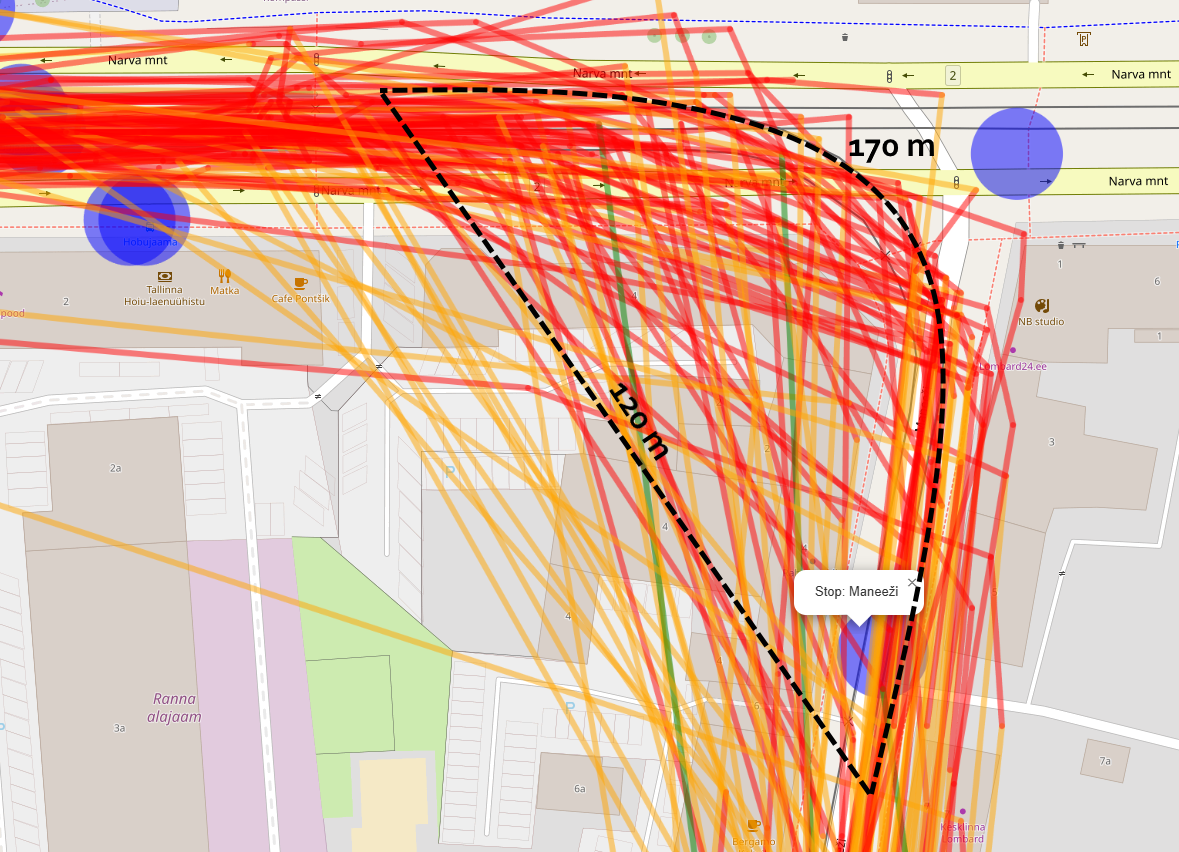
\includegraphics[width=.8\textwidth]{figures/Kurvsirgemaks.png} % Includes an image from the specified path, setting the width to 50% of the text width
    \caption{Trajektoorid lõikavad kurvi sirgemaks.} % Provides a caption for the figure, italicizing the text
    \label{fig:kurvsirgeks} % Sets a label for the figure to be referenced later
\end{figure}


Autor on siinse töö raames kogunud marsruutide andmeid ja kaalunud nende kasutamist täpsemate mõõtmiste saamiseks, kuid ei ole seda teinud suure töömahu tõttu.

Joonisel \ref{fig:kurvsirgeks} on näha, kuidas kiiruste arvutamisel ainult asukoha koordinaatidele tuginemine põhjustab olukordi, kus kurvid lõigatakse sirgemaks. Kuigi individuaalsed sektsioonid (sirge joon kahe mõõtmise vahel) näitavad õiget vahemaad, aega ja kiirust, siis sektsioonidest kokku pandud teekond võib hakata rohkete kurvide puhul vigast tulemust näitama. Reaalsuses on aga enamus marsruute suures osas võrdlemisi sirged  ja paljude kurvidega kohtades on ka ühistranspordi liikumiskiirused aeglasemad ja GNSS andmeid kogutakse läbitud vahemaa kohta rohkem kui sirgetel. See tähendab, et kurvide sirgeks lõikamine pole tegelikkuses nii suur probleem. Ning erinevalt eeltoodud Buenos Airesest, kus keskmiselt andis sõiduk oma asukohast teada iga 130 sekundi tagant ja ekstreemsematel juhtudel iga 10 minuti tagant, on Tallinna andmed palju järjepidevamad \cite{buenosAires}. Kiirused arvutatakse vaid siis, kui kahe andmepunkti vahe on 30 sekundit ehk 30 km/h liikuva sõiduki puhul keskmiselt iga 250 m tagant. Muid juhtumeid ignoreeritakse. See tähendab ka, et kaardile sobitamise algoritm ei ole hädavajalik. 
Peatükis \ref{section:valideerimine} analüüsiti erinevate liinide kiirusi ja leiti, et kurvide sirgeksvõtmise tõttu on keskmise kiiruse viga kuni 5\%. Autor pidas seda antud töö raames aksepteeritavaks, kuid edasiarenduste juures võiks sobitamise algoritmi rakendamist kaaluda.


\chapter{Tulemused}\label{chapter:results}
Töö tulemusena valmis avalikult kättesaadav veebirakendus \footnote{\url{https://tallinn.simplytobo.eu}}. Veebilehel valmis töö lõpuks mitu alamlehte. Töö lähtekood on avalikult kättesaadav. \footnote{\url{https://github.com/Tsarter/TallinnTransport}}

\section{Avalik andmebaas}

Kõik töö käigus kogutud andmed on avalikult kättesaadavad \footnote{\url{https://tallinn.simplytobo.eu/transport_data/}}. See võimaldab igal asjast huvitatud inimesel uurida Tallinna ühistransporti ja kuidas see on ajas muutunud. Antud töö raames ehitas autor mitmeid vahelehti just selle andmebaasi peale. Valminud lehtedest tuleb detailsemalt juttu järgmistes peatükkides. 

\section{Kiirused kaardil}\label{section:Kiirused-kaardil}

Pilte, kus kuvatud kiiruseid linnakaardil, on loodud näiteks Bostoni \cite{boston_woodruff_mbta_2011} ja Helsingi trammivõrgu jaoks \cite{jlf_tram_speeds}. Siin töös loodi sarnane interaktiivne kaart.

\begin{figure}[h!]
    \centering
    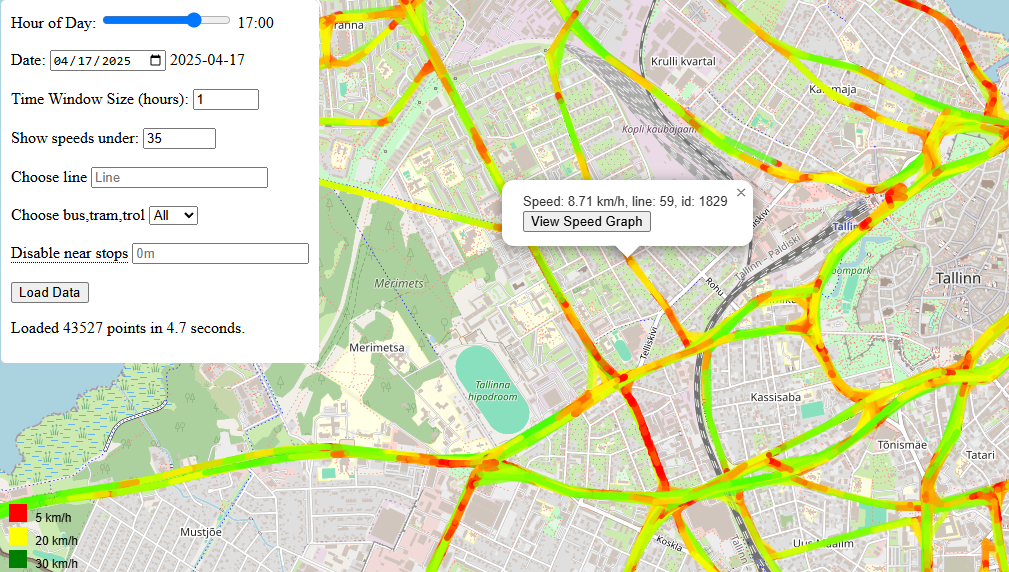
\includegraphics[width=0.8\textwidth]{figures/speedSegmentMap2.png}
    \caption{Kiirusi kuvav kaart. }
    \label{fig:Kiirustekaart}
\end{figure}

Joonisel \ref{fig:Kiirustekaart} on näha tallinna ühistranspordi sõidukite kiirusi neljandal aprillil aastal 2025 kella 17:00 - 18:00 vahel. Veebilehe kasutajal on võimalik valida kuupäev ja kellaaeg ning mitme tunni andmeid soovitakse näha. Aitamaks paremini näha aeglaseid kohti on võimalik välja filtreerida segmente kiiruse järgi. Soovides vaadelda konkreetset liini on seda võimalik teha sisestades vastava liini sümboli vastavasse kasti. Valides ka sõidukitüübi, saab tulemuse veelgi täpsemaks ja kuigi 1.november 2024 kadusid liinidelt trollid on antud rakenduses nende valimise võimalus olemas, kuna andmeid hakati koguma varem \cite{trollid}. Viimase võimalusena on võimalik välja jätta kõik segmendid, mis on ühistranspordi peatuste lähedal. Kasutaja saab sisestada numbri meetrites, mille järel ei näidata segmente, mis on lähemal. See aitab paremini näha fooride ja ristmike juures olevaid aeglaseid kohti. Andmete laadimiseks tuleb vajutada nuppu, mille järel saab näha kui palju andmeid laeti ja kui kiiresti.

Kollasega on segmendid, mille kiirus on 20 km/h lähedal. Seda kuna Lisa 2 andmetel on see ühissõidukite keskmine kiirus. Punasega on sellest allpool olevad kiirused ja rohelisega sellest ülevalpool olevad kiirused.

Igale kaardil olevale segmendile saab vajutada, et näha lisainformatsiooni. Selleks on kiirus, liin ja sõiduki identifikaator ning veelgi täpsemalt saab informatsiooni teada, kui vajutada nupule, kus on kirjas \textit{View Speed Graph}.

\section{Kiirused graafikul} 

Nägemaks paremini, kuidas kiirused päeva lõikes ühel liinil muutuvad, loodi vastav vaade. See avaneb, kui vajutada Joonisel \ref{fig:Kiirustekaart} mõne värvilise sektsiooni peale.

\begin{figure}[h]
    \centering
    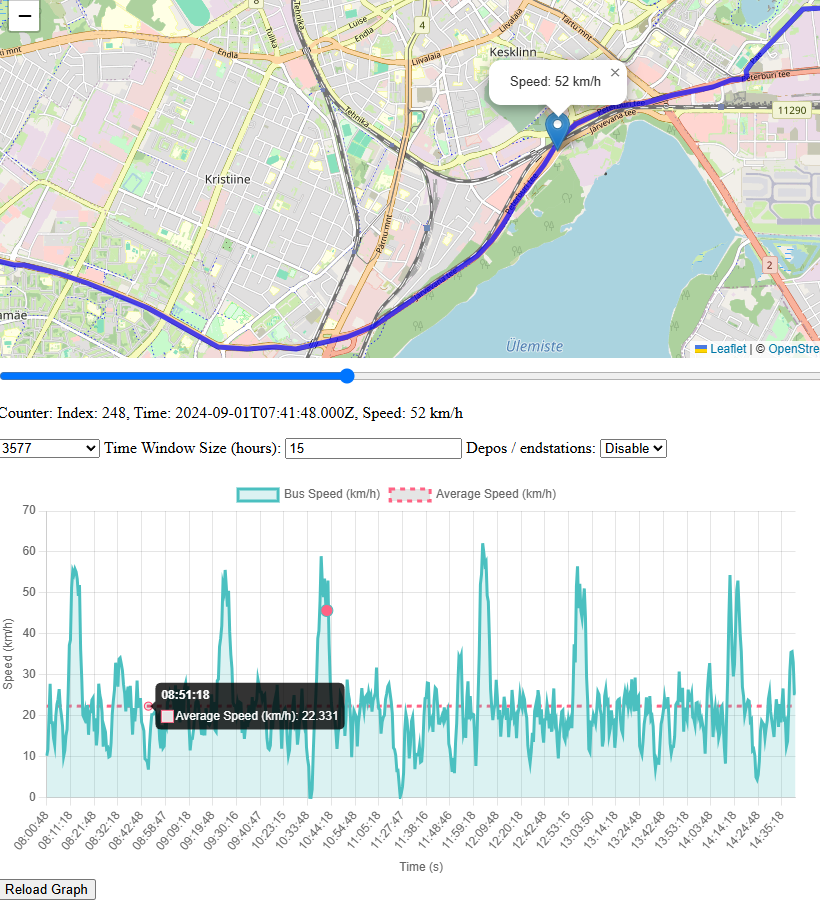
\includegraphics[width=0.8\textwidth]{figures/speedgraphDepos.png}
    \caption{Ühe sõiduki ühe päeva kiiruste graafik ja vastav kaart.}
    \label{fig:KiirusedGraafik}
\end{figure}

Joonisel \ref{fig:KiirusedGraafik} on näha bussiliini number 12 sõidukit identifikaatoriga 3577 1.septembril aastal 2024. Leheküljel on näha kaarti koos sõiduki marsruudiga, infot kellaaja ja hetkekiiruse kohta ning graafikut kiirustega. Graafikul on punase joonena kuvatud keskmist kiirust. 
Lehel on omavahel ühenduses kaart ja graafik. Lohistades sinist nuppu vasakule või paremale liigub punane täpp graafikul vastavasse kohta. Samal ajal liigub kaardil olev nupp kohta, kus sõiduk tol hetkel oli. Sedasi on näite puhul näha, et kui kiirused on suured, siis sõiduk asub Järvevana teel. Graafiku ajajoont jälgides on näha, et ajavahemikud ei ole ühtlased. Seda seetõttu, kuna lõpppeatustes ja depoos seismised on välja lõigatud. Juhul kui kasutaja soovib neid siiski näha on see võimalik seades \textit{Disable} nupu väärtuseks \textit{Enable}.


\section{Kahe punkti vaheline statistika} 

Saamaks paremat arusaama, kui kaua võtab aega ühistranspordil ühest kohast teise jõudmine, loodi vastav võimalus.

\begin{figure}[h!]
    \centering
    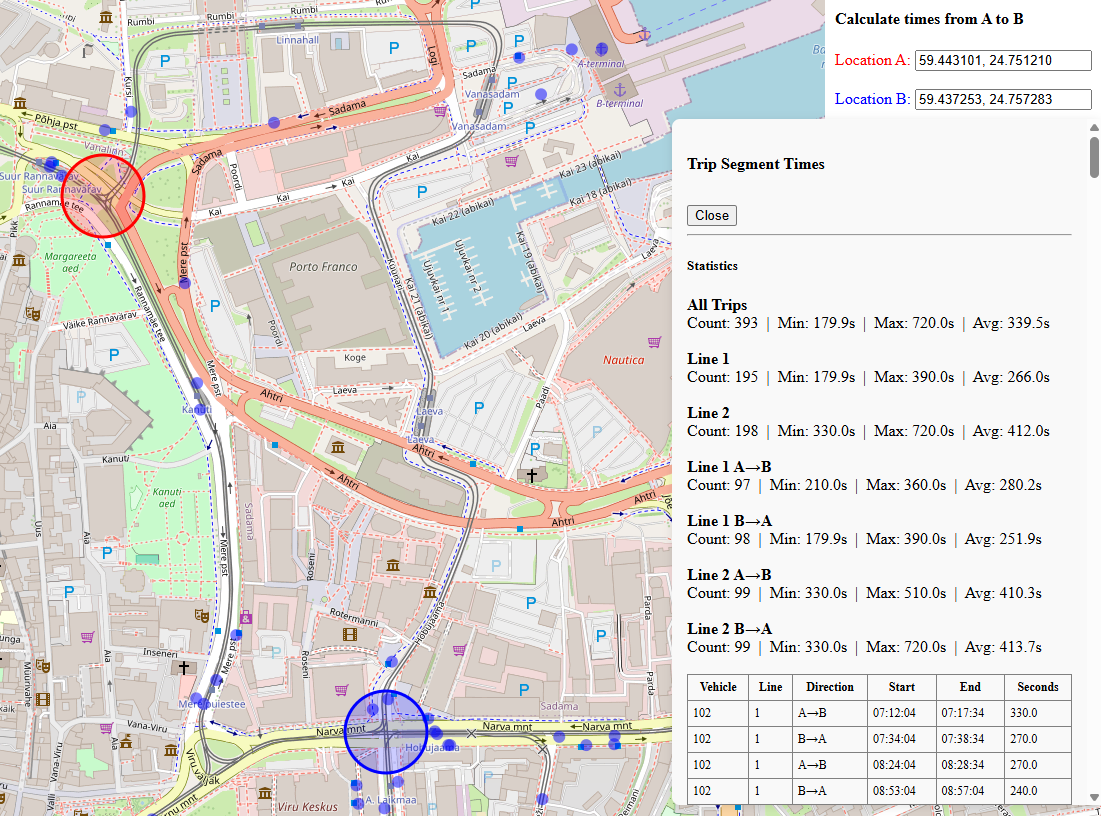
\includegraphics[width=0.8\textwidth]{figures/Liin1VsLiin2V2.png}
    \caption{Punkti A ja punkti B vahel liikunud sõidukite statistika.}
    \label{fig:Liin1VsLiin2V2}
\end{figure}

Võimalik on kaardile panna kaks ringi. Punane ring märgib punkti A ja sinine punkti B. Mõlema ringi raadius on 50 m. Andmebaasi päringu abil leitakse sõidukite teekonnad, mis läbisid neid kahte ringi. Statistika sektsioonis arvutatakse seejärel iga liini tuvastatud sõitude arv ning maksimaalne, minimaalne ja keskmine ajakulu. Lisaks näidatakse ka suuna põhiselt ehk punktist A punkti B kulunud aeg ja vastupidi. Kõige all on toodud ka kõik tuvastatud liikumised kahe punkti vahel tabelina välja. Selle tabeli saab kopeerida muude tarkvarasse, et sobivaid töötlusi veelgi teha. Näiteks saab vaadelda, kuidas ajakulu päeva lõikes muutub.


\section{Tallinna ühistranspordi keskmine kiirus}

Joonisel \ref{fig:KiirusedGraafik} on näha punast keskmise kiiruse joont. Selle info saab kätte iga liini kohta. Seda teadmist kasutades arvutati välja 2025. aasta märtsi sõidukite keskmised kiirused, mis on toodud välja Lisas 2.

Päringu tegemine võttis aega 20 minutit ja on seega aeglasema poolne. Autor on katsetanud eraldi tabeli tegemist taoliste päringute jaoks, mille tulemusel tehti sama päring alla sekundi. Kahjuks pole see lõplikult valmis ja on plaanis valmis teha tulevikus. Seetõttu pole keskmiste kiiruste infot ka avalikul veebilehel.

Katsetati ka muude päringute tegemist. Joonisel \ref{fig:nadalaKeskmine} on näha, kuidas tööpäeva alguses ja lõpus on kiirused madalamad kui tööpäeva keskel. Viimased kaks päeva on laupäev ja pühapäev ja seal on näha, et keskmine kiirus on päeva võrdluses ühtlasem. 
\begin{figure}[H]
    \centering
    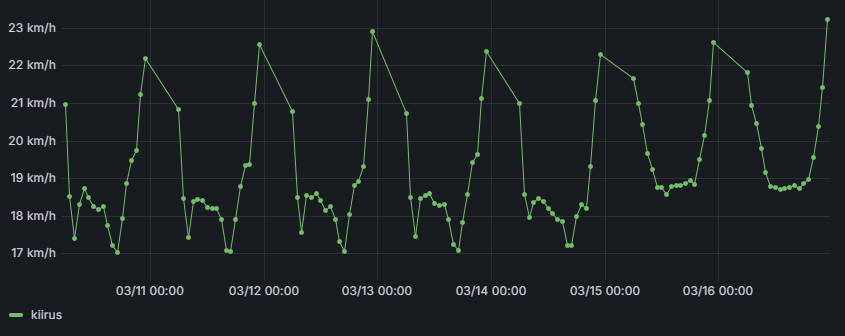
\includegraphics[width=0.9\textwidth]{figures/Kiirused5toopaeva2puhke.png}
    \caption{Kõikide ühissõidukite keskmiste kiiruste graafik ühe nädala vaates.}
    \label{fig:nadalaKeskmine}
\end{figure}





\section{Valideerimine}\label{section:valideerimine}

Tulemuste valideerimiseks võeti 4 bussi ja 1 trammi andmed. Kasutades Joonisel \ref{fig:KiirusedGraafik} näidatud tööriista pandi kirja, millal sõiduk algpeatusest väljus ja millal lõpppeatusesse jõudis. Google Earth'i \footnote{Liini pikkus~\url{https://earth.google.com/earth/d/1MccSsVoqKMNkUlBNQT4JodIoemFo2Ic8?usp=sharing}} abil leiti marsruudi ligikaudne pikkus.

Järgnevalt on näitena toodud ühe liini\footnote{Graafik leitav~\url{https://tallinn.simplytobo.eu/speedgraph/speedgraph.html?line=4&type=tram&vehicle_id=535&startTime=2025-04-14}} valideerimise protsess. 

\begin{longtable}{|l|c|c|c|c|c|c|}
\caption{14. aprillil trammiliinil 4 sõitnud trammi 535 sõidud.}
\label{tab:valideeringLiin4}\\ \hline % Sets a label for the table and starts the table with a horizontal line
\textbf{Väljumine}  &  \textbf{Saabumine} & \textbf{Aeg} & \textbf{Vahemaa} & \textbf{Kiirus} & \textbf{Alguspunkt} & \textbf{Sihtpunkt} \\ \hline
\endfirsthead
\hline
\textbf{Väljumine}  &  \textbf{Saabumine} & \textbf{Aeg} & \textbf{Vahemaa} & \textbf{Kiirus} & \textbf{Alguspunkt} & \textbf{Sihtpunkt} \\ \hline
\endhead
5:40:09 & 5:46:09  & 6 min & 2,1 km & 21,0 km/h & Pärnu mnt. depoo & Tondi \\ \hline
5:50:09 & 6:19:09  & 29 min & 7,6 km & 15,5 km/h & Tondi & Suur-Paala \\ \hline
6:31:39 & 6:59:39 & 28 min & 7,4 km & 16,1 km/h & Suur-Paala & Tondi \\ \hline
7:08:09 & 7:41:39  & 33,5 min & 7,6 km & 13,4 km/h & Tondi & Suur-Paala \\ \hline
7:48:09 & 8:19:09  & 32 min & 7,4 km & 14,1 km/h & Suur-Paala & Tondi \\ \hline
8:27:39 & 8:59:39  & 32 min & 7,6 km & 14,1 km/h & Tondi & Suur-Paala \\ \hline
9:19:39 & 9:49:09 & 29,5 min & 7,4 km & 15,2 km/h & Suur-Paala & Tondi \\ \hline
9:58:39 & 10:33:39  & 35 min & 7,6 km & 12,9 km/h & Tondi & Suur-Paala \\ \hline
10:49:39 & 11:19:09 & 29,5 min & 7,4 km & 15,2 km/h & Suur-Paala & Tondi \\ \hline
11:27:39 & 12:01:09  & 33,5 min & 7,6 km & 13,4 km/h & Tondi & Suur-Paala \\ \hline
12:10:39 & 12:40:39  & 30 min & 7,4 km & 15,0 km/h & Suur-Paala & Tondi \\ \hline
12:49:09 & 13:22:09  & 33 min & 7,6 km & 13,6 km/h & Tondi & Suur-Paala \\ \hline
13:31:09 & 14:01:09  & 30 min & 7,4\,km & 15,0 km/h & Suur-Paala & Tondi \\ \hline
14:05:39 & 14:12:09  & 6,5 min & 2,1 km & 19,4 km/h & Tondi & Pärnu mnt. depoo \\ \hline
\end{longtable}
Aeg tähendab siin aega, mis veedeti liinil olles. Iga marsruudi lõppu ja algusesse on seatud 75m suurune puhverala, mille sees olevaid mõõtmisi ei arvestata. See tähendab ka, et tabelis \ref{tab:valideeringLiin4} näitab vahemaa distantsi, mis läbiti ühest puhveralast teise jõudmiseks.

Käsitsi arvutamise järgi kulus 94,2 km läbimiseks 6 tundi ja 27 minutit. Keskmiseks kiiruseks saadi sel juhul 94,2 km / 6,45 h = 14.6 km/h. Automaatse skripti järgi sõideti 90,7 km ning liinil oldi 6 tundi ja 25 minutit ja keskmiseks kiiruseks saadi 14,2 km/h. 

Tegu on umbes 4 protsendilise erinevusega. Tegu ei ole suure eksimusega, kuid siiski on erinevus olemas. Nii automaatse skriptiga kui käsitsi saadud tulemused erinesid 2 minuti võrra ehk inimvea piires. 
Vahemaa erines 3,5 kilomeetriga. Seda mõningast viga võib põhjustada asjaolu, et asukohaandmed pole päris täpsed ehk kurvid võetakse sirgemaks. Joonisel \ref{fig:KiirusedGraafik} oleva tööriista järgi vaadeldi kurve. Näiteks Joonisel \ref{fig:kurvsirgeks} on viga kuskil 50 m. Arvestades, et tramm sõitis edasi-tagasi 12 korda, siis halvimal juhul tekkis ühes kurvis viga umbes 500 m. Trammiliinil 4 on kolm järsemat kurvi peatuste Lubja, Majaka ja Hobujaama lähedal, lisaks mitmeid laugemaid. Ehk 90 km peale võis sealt tekkida arvestatav viga. Selle lahendamiseks saaks asukohad tõsta teadaoleva marsruudi peale \cite{buenosAires}. Kahjuks jääb see töö mahust välja ja autor lepib teatud veaga kurvide arvutamisel.  

Järgnevalt valideeriti veel nelja erineva bussiliini andmeid. Lisas 2 on välja arvutatud 2025. aasta märtsi liinide liikumiskiirused. Selle abil valiti kõige kiirem bussiliin ehk 38, kõige aeglasem ehk 2 ja lisaks valiti ekspressliin 9, mille marsruut paistis ilma suuremate kurvideta. Bussiliin 81 valiti, kuna oli eelnevalt trolliliin.

\begin{longtable}{|l|c|c|c|c|c|c|}
\caption{Tulemuste valideerimine valitud sõidukite põhjal. Number 1 märgistab automaatse skripti tulemusi ja number 2 käsitsi valideerimisel saadud tulemusi. }
\label{tab:valideerimine}\\ \hline % Sets a label for the table and starts the table with a horizontal line
\textbf{Päev} & \textbf{Liin / id} & \textbf{Vahemaa 1} & \textbf{Vahemaa 2} & \textbf{Kiirus 1} & \textbf{Kiirus 2 } & \textbf{Viga} \\ \hline
\endfirsthead
\hline
\textbf{Päev} & \textbf{Liin / id} & \textbf{Vahemaa 1} & \textbf{Vahemaa 2} & \textbf{Kiirus 1} & \textbf{Kiirus 2 } & \textbf{Viga} \\ \hline
\endhead
2025-04-14 & 4 tramm / 535  & 90,7 km & 94,2 km & 14,2 km/h & 14,6 km /h & -3,7\% \\ \hline
2025-04-10 & 81 buss / 2669  & 214,9 km & 224,0 km & 16.0 km/h & 16.7 km/h & -4,2\% \\ \hline

2025-04-14 & 38 buss / 3320  & 126,1 km & 131,2 km & 25,9 km/h & 27.1 km /h & -4,4\% \\ \hline
2025-03-04 & 2 buss / 3535  & 155,8 km & 154,8 km & 15,6 km/h & 15,7 km /h & -0,6\% \\ \hline
2025-04-14 & 9 buss / 1813  & 160,1 km & 162,8 km & 22,8 km/h & 23,3 km /h & -2,1\% \\ \hline
\end{longtable}

Aegade võrdlusel ei leitud märkimisväärseid erinevusi ja seetõttu pole neid andmeid Tabelis \ref{tab:valideerimine}. Ainult bussiliini 2 mõõtmiste puhul oli märkimisväärne vahe, kus automaatne skript ei eemaldanud depoosse sõitu ja arvestas seda keskmise kiiruse arvutamisel. Kui see eemaldada tuleks vahemaa 149,8 km ja keskmine kiirus 15,2 km/h ning viga -3,2\%.
Liinide puhul esineb arvestav arv olukordi, kus depoost või depoosse sõitu ei lõigata välja. See muudab keskmist kiirust suuremaks. Kuna kurvide sirgeks lõikamine jälle vähendab keskmist kiirust, siis pikema perioodi jooksul need ilmselt mõnevõrra tühistavad üksteist. Samas ei saa sellele loota, kuna osade liinide lõpppeatused asuvad kohe depoo kõrval (nt bussiliin 9) ja seal ei tõsta depoosse sõit keskmist kiirust.

Bussiliini 38 puhul tuli viga kõige suurem, mis on tõenäoliselt seotud kurvilise ja kiire marsruudiga Pirita ja Viimsi teedel. Bussiliini 9 puhul tuli viga kõige väiksem ja see on ilmselt kuna Lasnamäelt Mustamäele sõidul pole järske kurve. 

Kuid üldpildis on kõik tulemused väga lähedal Lisas 2 leitud kiirustele. Kiiremad sõidukid ongi kiiremad ja aeglasemad aeglasemad. Seega peab autor leitud kiirusi õigeks, kuid paar protsenti liiga aeglaseks.

%\chapter{Second Chapter}\label{chapter:results}
%\input{chapters/second_chapter.tex}

\chapter{Analüüs}\label{chapter:discussion}

Siin peatükis tuuakse mõned näiteid, kuidas loodud tööriista saab kasutada ühistranspordi analüüsimiseks.

\section{Tulemuste võrdlus muude linnadega}


Tallinna ühistranspordi busside keskmiseks kiiruseks saadi 20 km/h. Trammide kiiruseks saadi 15 km/h ja mõlemat arvestades saadi keskmiseks kiiruseks 19,7 km/h.
Peatükis \ref{section:valideerimine} toodi välja, et kohati on kiirused kuni 5\% aeglasemad tegelikkusest ehk kuni 1 km/h.

Seda arvestades on Tabelis \ref{tab:maailmaKiirused} välja toodud Stockholmiga võrreldes Tallinna bussid 15 - 20\% aeglasemad.
Trammide kiirusi Stockholmis ei vaadeldud, kuid ülejäänud Euroopaga võrreldes on trammid kuskil 10\% aeglasemad. Seevastu Riiaga võrreldes on ühistransport sama kiire. Tundub, et seis ei ole kõige hullem kuid saaks paremini.

\section{Vanasadama tramm ja avalik arvamus} 

1. detsembril 2024 avati Tallinnas uus trammiliin \cite{err_trammiliin_2024}. Kuna endine trammiliin number 2 suunati läbi sadama sõitma, siis huvitas autorit, et kuidas see erineb trammiliin 1 ajakulust (Joonis \ref{fig:Liin1VsLiin2V2}).
 
Joonis \ref{fig:Liin1VsLiin2V2} kuvatud statistika juurest ilmnes, et läbi sadama sõitmine on aeglasem. Nimelt kulus trammiliinil 1 keskmiselt 4,5 minutit ja trammiliinil 2 keskmiselt 7 minutit kahe punkti vahel liikumiseks. See tähendab, et läbi sadama sõitmine muutis antud sektsioonil trammiliikluse 2,5 minutit aeglasemaks. 

Autor on olnud varasemast grupis nimega "Linnad ja liikuvus", mis on leitav Facebookist. Avalikku gruppi kuuluvad ja seal sõna võtavad näiteks Tallinna abilinnapead Kristjan Järvan, Peeter Pärtel Pere, Madle Lippus ja teised hetkel Tallinna ühistranspordi tulevikku kujundavad isikud.

Laskumata detailidesse nägi autor grupis postitust sadamatrammist  ja seal all kommentaare uue marsruudi rohkest ajakulust (eelnevalt sõitis tramm number 2 mööda mere puiesteed). Toodi välja, et tunnetuslikult olevat läbi sadama minemine kuni 10 minutit aeglasem, kuid puudusid konkreetsed andmeid.

Teades, et tegelikult oli trammiliini 2 teekond 2,5 minutit aeglasem  ei saanud seda mitte märkimata jätta. Joonisel \ref{fig:facebookiPostitus} ongi näha postituse alla tehtud kommentaar, kuhu lisati vastav tekst ja pilt. Autori hinnangul aitas see tuua faktilist tausta ja sellega koos aitas väikestviisi muuta avalikku arvamust. Sellistel väikestel mõjutustel võib pikemas plaanis olla arvestatav mõju ja sellega on ühtlasi ka osaliselt täidetud autori esialgne eesmärk. 
\begin{figure}[h!]
    \centering
    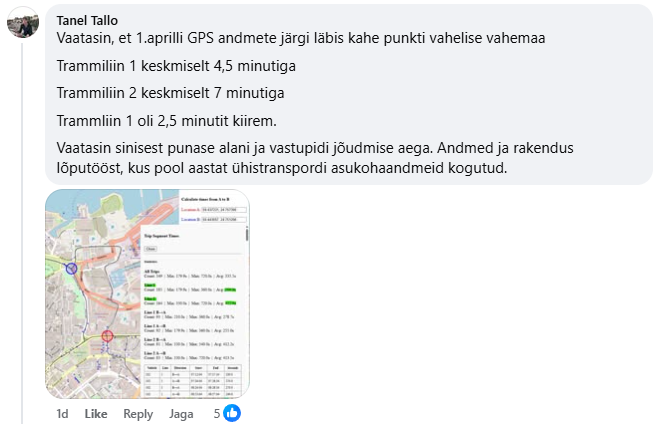
\includegraphics[width=0.8\textwidth]{figures/facebookiPostitus.png}
    \caption{Sotsiaalmeedia postituse kommentaar trammiliini 1 ja 2 võrdlusest.}
    \label{fig:facebookiPostitus}
\end{figure}

\section{Trammiliini 4 graafikus püsimine}

Graafikus püsimise täpsuse uurimiseks kasutati Joonisel \ref{fig:Liin1VsLiin2V2} olevat tööriista ning saadud andmed sisestati Google Spreadsheeti\footnote{\url{https://workspace.google.com/products/sheets/}}, mille abil saadi Joonis \ref{fig:kalevVaikePaala}.
\begin{figure}[h!]
    \centering
    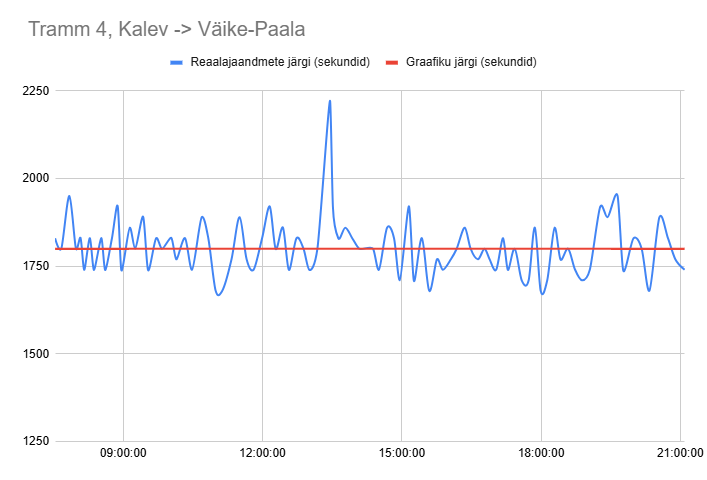
\includegraphics[width=0.8\textwidth]{figures/kalev-vaikepaala-kiirused.png}
    \caption{1. aprillil peatusest Kalev peatuseni Väike-Paala kulunud aeg trammiliinil 4. Tipptundide mõju ei ole näha, kella ühe paiku tekkis üks suurem hilinemine.}
    \label{fig:kalevVaikePaala}
\end{figure}
Graafiku järgi kulus kella 07:00 hommikust kuni poole kümneni õhtul alati 30 minutit Kalevist Väike-Paalasse sõitmiseks. Reaalajaandmete järgi kulus keskmiselt 30 minutit ja 4 sekundit. 73\% kordadest jõudis sõiduk kohale kuni 1-minutlise veaga. Ühel korral toimus suurem hilinemine, kus sõidukil kulus 7 minutit. Sõiduk peatus Paberi peatuse juures ligikaudu 5 minutit.

Üldiselt on graafikus püsimise täpsus hea. Päeva lõikes ei ole ka näha, et tipptundidel oleks ajakulu kuidagi suurem.

\section{Bussiliini ja ekspressliini võrdlus}

Bussiliin 83 ja ekspressliin 11 sõidavad sama marsruuti mööda Keemiast Estoniasse. Seetõttu olid need head liinid, mida võrrelda.
\begin{figure}[h!]
    \centering
    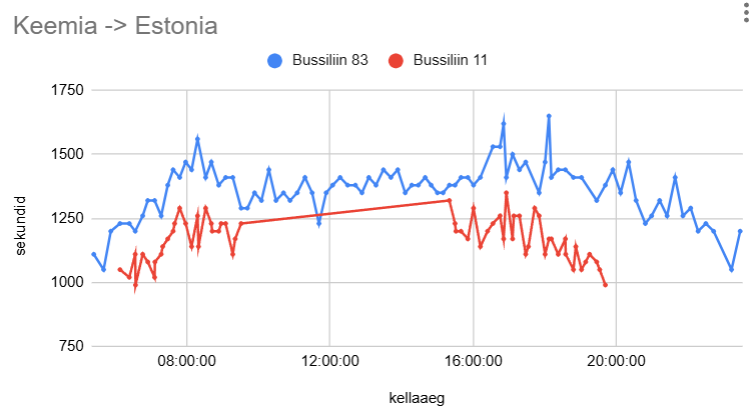
\includegraphics[width=0.8\textwidth]{figures/keemia-estonia.png}
    \caption{1. aprillil peatusest Keemia peatuseni Estonia kulunud aeg bussiliinidel 83 ja 11. Ekspressliin on kiirem.}
    \label{fig:keemiaEstonia}
\end{figure}

Nagu Jooniselt \ref{fig:keemiaEstonia} näha, siis ekspressliin on kiirem. Kuigi kella viiesel tipptunnil on näha, et vahe ei ole alati väga suur. Kahel korral oli vahe 1 minut ja kahel korral 1,5 minutit. Bussiliini 83 juures on varahommikul ja hilisõhtul  ajakulu märksa väiksem. Liikluse tihenedes muutus see suuremaks. 

Vaadeldes ainult aegu, millal mõlemad sõitsid, siis hommikul oli ekspressliin keskmiselt 3,5 minutit kiirem ja õhtul 4,5 minutit kiirem. Keskmiselt oli ekspressliin 17\% kiirem. Tulemused on mõneti üllatavad, kuna vahe polegi nii suur kui eeldada. Mustamäe osas peatuvad mõlemad liinid suuresti samades peatustes ja võitu eriliselt pole. Kuid, kui vaadelda viimasest Mustamäe peatusest Siili peatuseni Estonia, siis on ekspressliin ligi 30\% kiirem ja ajaliselt keskmiselt 4 minutit.

\section{Teelõigu võrdlus}
Võimalik on ka saada ülevaade tervest teelõigu ajakulust päeva lõikes.
Näiteks uuriti Pärnu maantee Kesklinna jäävat osa.

\begin{figure}[h!]
    \centering
    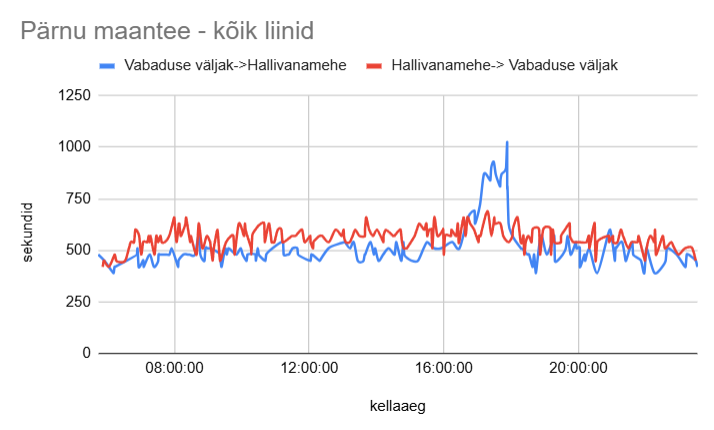
\includegraphics[width=0.8\textwidth]{figures/parnumnt.png}
    \caption{1. aprillil peatuse Hallivanamehe juurest Vabaduse väljaku ristini kulunud aeg ühissõidukitel. Linnast väljudes on tipptunni mõju näha, linna sisse sõites aga mitte.}
    \label{fig:parnumnt}
\end{figure}

Nagu Jooniselt \ref{fig:parnumnt} näha, siis päeva jooksul oli suund Vabaduse väljaku poole pidevalt veidi aeglasem, kuid tipptunnil ajakulu ei suurenenud. Seevastu Vabaduse väljaku poolt tulles oli ajakulu suurem 16:30 ja 18:00 vahel. Sel ajaperioodil kulus keskmiselt 5 minutit rohkem kui sellele eelneval ajal. Ajakulu kasvas 8 minuti pealt 13 minuti peale ehk 60\%. 

Kasutaja poolest on ilmselt parem pidevalt ühtlane kiirus, kui tipptunnil  suurem ajakulu. Peatükis \ref{section:Kiirused-kaardil} kirjeldatud tööriista abil vaadeldi, et sisuliselt kogu teekond Pärnu maantee viaduktist kuni Hallivanameheni oli tipptunnil ühissõidukile punane. Täies pikkuses ühissõidukiraja loomine on hetkel ilmselt liiga suur ettevõtmine, kuid kui tuleviks peaks tramm Järve keskuseni sõitma hakkama, siis oleks  antud andmete järgi mõistlik ehituse käigus ka ühisrada planeerida \cite{err_jarve_tramm_2024}.

Kaardirakenduse Waze\footnote{\url{https://www.waze.com/}} järgi võtab autoga Vabaduse väljakult Hallivanameheni jõudmine tipptunnil aega kuskil 10 minutit. Jättes kõrvale bussipeatusesse kõndimise ja sõiduki ootamise, siis bussiraja olemasolul oleks tipptunnil buss antud teekonnal autost tõenäoliselt kiirem.  See võiks muuta Pärnu maanteed mööda liikuvaid ühistranspordiliine atraktiivsemaks. Seeläbi tõuseks Pärnu maantee läbilaskevõime, kuna bussidesse mahub rohkem inimesi.

\section{Edasiarenduste võimalused}

Töö raames loodud lahendused aitavad visualiseerida üldist pilti. Täpsemate tulemuste nägemiseks saaks teha mitmeid edasiarendusi.

Sõidugraafikute integreerimise tulemusena saaks näha, millistel liinidel ja mis peatustes toimub kõige rohkem kõrvalekaldeid. Saaks näha kaua keskmiselt üks sõiduk peatuses peatub ja kas Tallinnas on kohti, kus see on keskmisest oluliselt kõrgem.

Ühe lisana oleks võimalik uurida reaalajaandmete järgi busside kobardumist. See tähendab, kui bussid saabuvad samasse peatusesse samal ajal. Saaks näha, mis peatustes või lõikudel seda kõige rohkem juhtub.

Keskmiste kiiruste arvutamise täpsuse tõstmiseks saaks sobitada sissetulevaid sõidukite asukohti reaalsete liinide peale (\textit{map matching}). See võimaldaks vältida kurvide sirgeksvõtmisest tulenevaid probleeme, kuid võib suurendada probleeme juhul, kui teel oli takistus ja sõiduk pidi minema teist teed pidi. 

Kuigi iga 30 sekundi tagant kogumine tähendas siin töös kiiremaid päringuid, lihtsamat töötlemist ja väiksemat andmebaasi, siis võiks kaaluda tihedamalt kogumist. Näiteks iga 10 sekundi tagant kogumine võiks anda parema täpsuse. Loodud andmebaasi struktuur ja andmed tuleks viia GTFS standardile vastavaks. Selliselt oleks andmebaasi andmeid kolmandatel osapooltel lihtsam kasutada.

Praegu kasutuses olev PostGIS andmebaasi laiend võimaldab küll teha geograafilisi päringuid lihtsasti, kuid sõidukite sõitude analüüsimiseks saaks lisada rohkemate lisadega laiendit nimega MobilityDB\footnote{\url{https://mobilitydb.com/}}. See on spetsiaalselt loodud järjestatud geograafiliste aegridade analüüsimiseks. See ei asenda PostGIS laiendit, kuid võimaldaks lisafunktsioone. Näiteks hetkel saab lihtsasti kätte sõiduki läbitud geograafiliste asukohtade jada \footnote{\url{https://postgis.net/docs/ST_MakeLine.html}}, kuid ilma ajalise mõõtmeta. MobilityDB lahendaks selle mure, kuna võimaldab lisada igale asukohale näiteks kellaaja ja kiiruse. Lisaks, kui praegu on sõiduki asukohaandmed andmebaasis olemas kella 14:30:00 ja  14:30:30 jaoks, siis MobilityDB abil saaks leida eeldatava kiiruse ja asukoha ükskõik millal, ka kell 14:30:15. Päringute puhul ei oleks enam oluline teada konkreetset aega ega asukohta.



\chapter{Kokkuvõte}\label{chapter:summary} 
Töö eesmärgiks oli visualiseerida muidu raskesti arusaadavaid ühistranspordi  asukohaandmeid ja muuta need paremini kättesaadavaks.

Tegemise käigus ilmnes, kui palju keerulisem on suuremahuliste andmete hoiustamine. See põhjustas mitmeid kitsaskohti, mille käigus tuli proovida mitmeid andmete hoiustamise viise. Vastasel korral oleks osade päringute tegemine paari sekundi asemel võtnud mitusada korda rohkem aega. Töö algusega võrreldes suudeti andmete kogumisel andmemahtu vähendada 90\% andmete sisu muutmata.

Töö algul seadsin paika kaks küsimust. Esiteks, et mis on liinil sõitvate sõidukite liikumiskiirused. 
Sellele saadi vastus läbi graafilise kaardi, kust on näha sõidukite liikumiskiirused. Lisaks on sinna lisatud võimalused filtreerida andmeid selliselt, et on näha vaid huvipakkuv liin, kellaaeg, ajaakna suurus ja on võimalus jätta välja kiirused bussipeatuste lähedal. Arvutati ka välja ühe kuu keskmine liikumiskiirus iga liini kohta eraldi.

Teiseks, et kui suured on liinil sõitvate sõidukite hilinemised.
Selle saavutamine täielikult ei õnnestunud. Sõidugraafikute tõlgendamisega esines probleeme ja alles töö lõpus leiti teoorias sobiv lahendus. Sellegipoolest näidati töös võimalusi hilinemiste nägemiseks. Seda siis, kui kasutada ühte loodud tööriista, kus saab valida geograafilised asukohad ja vaadelda ajakulu nende vahel.

Lõppkokkuvõttes valmis veebileht, mis on avalikult kättesaadav, võrdlemisi kiire ja interaktiivne. Seal on mitmeid võimalusi Tallinna ühistranspordi asukohaandmete vaatlemiseks ja analüüsimiseks. Kõik kogutud andmed on avalikud kättesaadavad ja igaüks saab sinna peale ennast huvitava veebilehe ehitada. Selliselt võib tööst kasu olla nii ühistranspordihuvilistel, linnaplaneerijatel kui ka avalikusel.






\zlabel{lastpagetocount}        % DO NOT REMOVE! Used for counting number of pages of main text


\pagebreak % Content that follows starts on the new page
\phantomsection % Creates linkable section without placing visible content
\addcontentsline{toc}{chapter}{\referencesTitle} % adds a new chapter entry labeled "Kasutatud kirjandus" to TOC
\printbibliography[title=\referencesTitle] % The command pulls from the .bib file and and formats the output

\pagebreak
\phantomsection
\appendix % This command signals that the following sections will be appendices.

% \addcontentsline{toc}{chapter}{Appendices}
% \chapter*{Appendices}
\renewcommand{\thechapter}{\arabic{chapter}} % This command redefines how chapter numbers are displayed.

% Licence
% Footnote for a licence
% This command adds an entry to the table of contents (TOC).
\addcontentsline{toc}{chapter}{\appendixTitle~1 -- \licenceTitle}\label{chapter:licence}

% This is the title of the licence section, which is being displayed as a chapter heading and it adds a footnote at the end of the chapter title
{\let\clearpage\relax\chapter*{\appendixTitle~1 -- \licenceTitle\footnote{\licenceFootnote}}}
% Generates the list of supervisors. Do not edit
\newcommand{\supervisorList}[1]
{
  \ifthenelse{\equal{#1}{[Co-Supervisor's Name]}}{\mbox{\supervisorName}}{\mbox{\supervisorName}~and \mbox{\cosupervisorName}}
}

\newcommand{\supervisorListEst}[1]
{
  \ifthenelse{\equal{#1}{[Kaasjuhendaja nimi]}}{\mbox{\supervisorNameEst}}{\mbox{\supervisorNameEst}~and \mbox{\cosupervisorNameEst}}
}

% The licence should be automatically filled, please double check that everything is fine before submitting
\ifthenelse{\equal{\lang}{ENG}}{
  \ifthenelse{\equal{\authorNameTwo}{[Second Author name]}}
  {
  I \authorName

  \begin{enumerate}[label*=\arabic*.]
      \item Grant Tallinn University of Technology free licence (non-exclusive licence) for my thesis ``\thesisTitleEng'', supervised by \supervisorList{\cosupervisorName}
      \begin{enumerate}[label*=\arabic*.]
          \item to be reproduced for the purposes of preservation and electronic publication of the graduation thesis, incl. to be entered in the digital collection of the library of Tallinn University of Technology until expiry of the term of copyright;
          \item to be published via the web of Tallinn University of Technology, incl. to be entered in the digital collection of the library of Tallinn University of Technology until expiry of the term of copyright
      \end{enumerate}
      \item I am aware that the author also retains the rights specified in clause 1 of the nonexclusive licence.
      \item I confirm that granting the non-exclusive licence does not infringe other persons' intellectual property rights, the rights arising from the Personal Data Protection Act or rights arising from other legislation.
  \end{enumerate}
  }
  {
    We\ifthenelse{\equal{\authorNameThree}{[Third Author name]}}{ % Two authors
          \authorName~and~\authorNameTwo
        }{
          \authorName,~\authorNameTwo~and~\authorNameThree
        }

    \begin{enumerate}[label*=\arabic*.]
        \item Grant Tallinn University of Technology free licence (non-exclusive licence) for our thesis ``\thesisTitleEng'', supervised by \supervisorList{\cosupervisorName}
        \begin{enumerate}[label*=\arabic*.]
            \item to be reproduced for the purposes of preservation and electronic publication of the graduation thesis, incl. to be entered in the digital collection of the library of Tallinn University of Technology until expiry of the term of copyright;
            \item to be published via the web of Tallinn University of Technology, incl. to be entered in the digital collection of the library of Tallinn University of Technology until expiry of the term of copyright
        \end{enumerate}
        \item We are aware that the authors also retain the rights specified in clause 1 of the nonexclusive licence.
        \item We confirm that granting the non-exclusive licence does not infringe other persons' intellectual property rights, the rights arising from the Personal Data Protection Act or rights arising from other legislation.
    \end{enumerate}
  }
} {
  \ifthenelse{\equal{\authorNameTwo}{[Second Author name]}}
  {
    Mina, \authorNameEst

    \begin{enumerate}[label*=\arabic*.]
        \item Annan Tallinna Tehnikaülikoolile tasuta loa (lihtlitsentsi) enda loodud teose ``\thesisTitleEst'', mille juhendaja on \supervisorListEst{\cosupervisorNameEst}
        \begin{enumerate}[label*=\arabic*.]
            \item reprodutseerimiseks lõputöö säilitamise ja elektroonse avaldamise eesmärgil, sh Tallinna Tehnikaülikooli raamatukogu digikogusse lisamise eesmärgil kuni autoriõiguse kehtivuse tähtaja lõppemiseni;
            \item üldsusele kättesaadavaks tegemiseks Tallinna Tehnikaülikooli veebikeskkonna kaudu, sealhulgas Tallinna Tehnikaülikooli raamatukogu digikogu kaudu kuni autoriõiguse kehtivuse tähtaja lõppemiseni.
        \end{enumerate}
        \item Olen teadlik, et käesoleva lihtlitsentsi punktis 1 nimetatud õigused jäävad alles ka autorile.
        \item Kinnitan, et lihtlitsentsi andmisega ei rikuta teiste isikute intellektuaalomandi ega isikuandmete kaitse seadusest ning muudest õigusaktidest tulenevaid õigusi.
    \end{enumerate}
  }
  {
    Meie,\ifthenelse{\equal{\authorNameThree}{[Third Author name]}}{ % Two authors
              \authorName~ja~\authorNameTwo
          }{
              \authorName,~\authorNameTwo~ja~\authorNameThree
          }       

    \begin{enumerate}[label*=\arabic*.]
        \item Anname Tallinna Tehnikaülikoolile tasuta loa (lihtlitsentsi) enda loodud teose ``\thesisTitleEst'', mille juhendaja on \supervisorListEst{\cosupervisorNameEst}
        \begin{enumerate}[label*=\arabic*.]
            \item reprodutseerimiseks lõputöö säilitamise ja elektroonse avaldamise eesmärgil, sh Tallinna Tehnikaülikooli raamatukogu digikogusse lisamise eesmärgil kuni autoriõiguse kehtivuse tähtaja lõppemiseni;
            \item üldsusele kättesaadavaks tegemiseks Tallinna Tehnikaülikooli veebikeskkonna kaudu, sealhulgas Tallinna Tehnikaülikooli raamatukogu digikogu kaudu kuni autoriõiguse kehtivuse tähtaja lõppemiseni.
        \end{enumerate}
        \item Oleme teadlikud, et käesoleva lihtlitsentsi punktis 1 nimetatud õigused jäävad alles ka autoritele.
        \item Kinnitame, et lihtlitsentsi andmisega ei rikuta teiste isikute intellektuaalomandi ega isikuandmete kaitse seadusest ning muudest õigusaktidest tulenevaid õigusi.
    \end{enumerate}
  }
}

% Defaults to current date. If you want a specific date, replace \signaturedate with hardcoded value
\signatureDate
 % This command imports the content from an external file

% Other appendices
% NOTE: Appendix 1 is always the non-exclusive licence.
% Therefore, your appendices need to start from 2.

\clearpage % Forces a page break, ending the current page and starting a new one
\phantomsection % Creates a section that doesn't produce visible content but is needed for hyperlinks
\addcontentsline{toc}{chapter}{\appendixTitle~2 -- Ühistranspordi liinide keskmised kiirused märtsis 2025}\label{chapter:appendix-something} % Adds an entry to the table of contents
\chapter*{\appendixTitle~2 -- Ühistranspordi liinide keskmised kiirused märtsis 2025} % Creates an unnumbered chapter

5 trammiliini ja  68 bussiliini keskmised kiirused märtsis 2025.

\begin{longtable}{|l|c|c|c|} \hline
 \textbf{Keskmine kiirus (km/h)}  & \textbf{Liini number}  & \textbf{Liik} \\
\hline
\endfirsthead
\hline
\textbf{Keskmine kiirus (km/h)} & 
\textbf{Liini number} & \textbf{Liik} \\
\hline
\endhead
19,7 & kõik & kõik\\ \hline
15,0 & kõik & trammid\\ \hline
20,0 & kõik & bussid\\ \hline
14,1	&	3	&	tramm	\\ \hline
14,3	&	4	&	tramm	\\ \hline 
15,2	&	5	&	tramm	\\ \hline
15,2	&	2	&	tramm	\\ \hline
16,3	&	1	&	tramm	\\ \hline
15,7	&	2	&	buss	\\ \hline
16	&	3	&	buss	\\ \hline
16,1	&	81	&	buss	\\ \hline
16,7	&	40	&	buss	\\ \hline
17	&	39	&	buss	\\ \hline
17,2	&	85	&	buss	\\ \hline
17,4	&	73	&	buss	\\ \hline
17,5	&	35	&	buss	\\ \hline
17,6	&	23	&	buss	\\ \hline
17,6	&	84	&	buss	\\ \hline
17,7	&	83	&	buss	\\ \hline
17,9	&	15	&	buss	\\ \hline
18,1	&	26A	&	buss	\\ \hline
18,3	&	37	&	buss	\\ \hline
18,3	&	61	&	buss	\\ \hline
18,4	&	16	&	buss	\\ \hline
18,5	&	55	&	buss	\\ \hline
18,5	&	44	&	buss	\\ \hline
18,6	&	28	&	buss	\\ \hline
18,6	&	72	&	buss	\\ \hline
18,7	&	33	&	buss	\\ \hline
18,8	&	60	&	buss	\\ \hline
18,9	&	24	&	buss	\\ \hline
19	&	31	&	buss	\\ \hline
19	&	66	&	buss	\\ \hline
19,1	&	67	&	buss	\\ \hline
19,2	&	18	&	buss	\\ \hline
19,3	&	36	&	buss	\\ \hline
19,4	&	26	&	buss	\\ \hline
19,5	&	59	&	buss	\\ \hline
19,5	&	58	&	buss	\\ \hline
19,6	&	10	&	buss	\\ \hline
19,6	&	20	&	buss	\\ \hline
19,6	&	11	&	buss	\\ \hline
19,8	&	50	&	buss	\\ \hline
19,9	&	20A	&	buss	\\ \hline
19,9	&	32	&	buss	\\ \hline
20,1	&	14	&	buss	\\ \hline
20,2	&	29	&	buss	\\ \hline
20,2	&	63	&	buss	\\ \hline
20,3	&	42	&	buss	\\ \hline
20,3	&	18A	&	buss	\\ \hline
20,4	&	54	&	buss	\\ \hline
20,5	&	62	&	buss	\\ \hline
20,5	&	41B	&	buss	\\ \hline
20,6	&	41	&	buss	\\ \hline
20,6	&	25	&	buss	\\ \hline
21	&	21B	&	buss	\\ \hline
21,2	&	13	&	buss	\\ \hline
21,2	&	5	&	buss	\\ \hline
21,4	&	27	&	buss	\\ \hline
21,4	&	1	&	buss	\\ \hline
21,4	&	21	&	buss	\\ \hline
21,4	&	7	&	buss	\\ \hline
21,5	&	8	&	buss	\\ \hline
22,2	&	45	&	buss	\\ \hline
23	&	30	&	buss	\\ \hline
23	&	49	&	buss	\\ \hline
23,1	&	12	&	buss	\\ \hline
23,2	&	4	&	buss	\\ \hline
23,2	&	6	&	buss	\\ \hline
23,3	&	9	&	buss	\\ \hline
23,3	&	21A	&	buss	\\ \hline
23,5	&	46	&	buss	\\ \hline
23,6	&	48	&	buss	\\ \hline
23,8	&	34	&	buss	\\ \hline
24,8	&	57	&	buss	\\ \hline
25,4	&	38	&	buss	\\ \hline
\end{longtable} 
 % Includes the content of the specified file (appendix-something.tex)
%\clearpage
%\phantomsection
%\addcontentsline{toc}{chapter}{\appendixTitle~3 -- Something %Else}\label{chapter:appendix-something-else}
%\chapter*{\appendixTitle~3 -- Something Else}
%\input{appendices/appendix-something-else.tex}


\end{document}
